\documentclass[preprint2,tighten]{aastex62}
\pdfoutput=1 %for arXiv submission
\usepackage{amsmath,amstext}
\usepackage[T1]{fontenc}
\usepackage{txfonts} %use times font for math
\usepackage[figure,figure*]{hypcap} %Figure refs go figures
\usepackage{bm}

\renewcommand*{\sectionautorefname}{Section} %for \autoref
\renewcommand*{\subsectionautorefname}{Section} %for \autoref

\newcommand*{\kms}{\,km~s$^{-1}$}
\newcommand{\todo}[1]{{\bf \textcolor{red}{ #1}}}

\shorttitle{}
\shortauthors{the IQ (Isolated \& Quenched) collaboratory}

\begin{document}


\title{Paper I: The Main Sequence of Simulated Galaxies}
%\title{Distributions of star-forming galaxies: predictions}
\author{ChangHoon Hahn}
\altaffiliation{changhoonhahn@lbl.gov}
\affil{Lawrence Berkeley National Laboratory, 1 Cyclotron Rd, Berkeley CA 94720, USA}
\affil{Berkeley Center for Cosmological Physics, University of California, Berkeley, CA 94720, USA}
\author{Tjitske K. Starkenburg}
\affil{Flatiron Institute, 162 Fifth Avenue, New York NY 10010, USA}
\author{Claire Dickey}
\affil{Yale University}

\author{IQ collaboratory (in alphabetical order)}
\affil{various}

\begin{abstract}
Principled comparisons between the galaxy populations of simulations and 
observations play a pivotal role in validating our theories of galaxy 
formation and evolution. %are necessary to validate our theories of galaxy formation and  evolution. 
Key features in galaxy property-space like the star forming main sequence
(SFMS), which track %encapsulate %the evolution of 
star forming galaxies since $z<2$,
and a consistent  way to identify them are critical for such comparisons. 
We present a data-driven approach to fitting the SFMS using Gaussian 
Mixture Models that can be flexibly applied to a wide range of star 
formation to stellar mass relations down to $M_*{\sim}10^{8}M_\odot$. %and across four orders of magnitude in stellar mass.
Using this method, we identify the SFMS of central galaxies in 
the Illustris, EAGLE, and MUFASA hydrodynamic simulations, the Santa Cruz 
Semi-Analytic Model simulation, and observations from the Sloan Digital 
Sky Survey Data Release 7 and the NASA Sloan Atlas. Among our simulations, 
we find discrepancies on the order of a magnitude in the amplitudes of the 
SFMSs. In addition, our fitting method also identifies subpopulations 
that correspond to quenched, transitioning, and star-burst galaxies. We 
find overall consistent subpopulations among our hydrodynamic 
simulations but not with the semi-analytic model. Using these subpopulations, 
we find that the quiescent fractions of the hydrodynamic simulations do 
not reproduce measurements from observations. Moreover, in \emph{all} of the 
simulations we find a significant fraction of quenched galaxies at 
$M_* < 10^9M_\odot$, in conflict with the literature. %below the established \cite{geha2012} threshold. 
The SFMS fitting method we present provides a data-driven framework to 
consistently compare galaxy samples from both simulations and observations. 
\end{abstract}
\keywords{cosmology: observations --- galaxies: star formation --- galaxies:statistics}

\section{Introduction}
Large galaxy surveys of the past decade such as the Sloan Digital Sky 
Survey~\citep[SDSS;][]{york2000}, have firmly established the major 
trends of galaxies in the local universe. Galaxies %in the properties 
broadly fall into two populations: quiescent galaxies with little star
formation that are red in color with elliptical morphologies and star 
forming galaxies with significant star formation that are blue in color 
with disk-like morphologies 
(\citealt{kauffmann2003, blanton2003, baldry2006, taylor2009, moustakas2013}; 
for a recent review see~\citealt{blanton2009}). 
Star forming galaxies, furthermore, are found to have a tight relationship 
between their star formation rates (SFR) and stellar masses placing them
on the so-called ``star formation main sequence'' (hereafter 
SFMS)~\citep[\emph{e.g.}][]{noeske2007, daddi2007, salim2007}.

%Star forming galaxies are found to have tightly correlated 
%star formation rates (SFR) and stellar 
%masses~\citep[\emph{e.g.}][\todo{more}]{noeske2007, daddi2007, salim2007}.

% Galaxy evolution from the perspective of the SFMS. 
In fact, this sequence of star forming galaxies is found in observations 
well beyond the local universe out to $z > 2$~\citep{wang2013, schreiber2015}.
But more than its persistence, the SFMS plays a crucial role in characterizing 
the evolving galaxy population. The most dramatic transformations of 
galaxies over the past $10\,\mathrm{Gyr}$ can be described by the SFMS. 
For instance, the decline in the number density of massive 
star forming galaxies and the accompanying growth in number density of 
quiescent galaxies reflects the cessation of star formation in 
star forming galaxies migrating off of the 
SFMS~\citep{blanton2006, borch2006, bundy2006, moustakas2013}. 
Similarly, the cosmic decline in star formation~\citep{hopkins2006,
behroozi2013a, madau2014} reflects the overall decline of star 
formation of the SFMS~\citep{schreiber2015}. 

%in the continuing effort to understand  the physical processes governing galaxy formation and evolution, 
Numerical simulations today \emph{qualitatively} reproduce the SFMS and 
similar global relations of galaxy properties 
(\emph{e.g.}~\citealt{ vogelsberger2014,genel2014, schaye2015, dave2017}; 
for a recent review see~\citealt{somerville2015}). These hydrodynamic and 
semi-analytic simulations each seek to capture the complex physics of 
gas heating and cooling, star formation, stellar feedback, chemical 
evolution, black hole formation and evolution, and AGN feedback using 
their distinct sub-grid model prescriptions. Both as an effort to shed 
light on the underlying physics and to valid their simulations, many 
works have already compared simulations to 
observations~\citep[\emph{e.g.}][]{vogelsberger2014, 
genel2014, torrey2014, sparre2015, schaye2015, bluck2016, dave2017}. 
These works, however, primarily focus on comparing one specific simulated 
galaxy sample to one or a few observational datasets. Extending such 
comparisons to include multiple simulations, observations, and a 
consistent framework for comparing the data-sets would allow us to make 
detailed comparison of the different sub-grid models and thereby provide 
key insights into the physics that govern galaxy formation and evolution.  

%At the same time a general understanding of the key physical processes  in the formation and evolution of galaxies has arisen from numerical simulations. Global galaxy properties, correlations, and distribution  functions can nowadays (approximately) be reproduced by hydrodynamical,  and semi-analytical cosmological and zoom simulations that include gas  heating and cooling, star formation and stellar feedback, chemical  evolution, and black hole formation, evolution, and AGN feedback. Due to the immense range in scales that needs to be covered by these simulations, many  of these processes are implemented using sub-grid models, that vary in their prescriptions depending on simulation method, code, and resolution. Even  though the effects can be similar, the detailed processes in these feedback schemes may differ, for example whether feedback due to AGN in simulations  is most effective in suppressing cold gas accretion and star formation when modeled as thermal, kinetic, or radiative feedback, or any combination of  these depending on central black hole and galaxy properties \todo{refs}.  Present-day galaxy formation models do qualitatively reproduce the evolution of the SFMS and similar global scaling relations \citep{SomervilleDave2015ARAA, vogelsberger2014,genel2014, schaye2015, dave2016, dave2017}\todo{and more}. Many comparisons of the SFMS between observations and simulations have been made, but these usually focus on comparing one specific simulated galaxy sample to one or a few observational datasets \citep{vogelsberger2014,genel2014, schaye2015, dave2016,bluck2016, torrey2014,sparre2015}\todo{and more}. 

%Nonetheless, with the key role that starforming galaxies play in our understanding of the formation and evolution of galaxies, the SFMS is an important relation to compare to for simulations. Moreover, the SFMS can form a tool to understand the starforming and non-starforming galaxy populations and the processes that create those. Therefore we argue that a comparing the galaxy populations in the SFR-$M_{\star}$ plane between different simulations that vary in technique and in descriptions of key physical processes, is important. The SFMS serves as a key feature in galaxy sample data for comparison. Therefore in this paper we compare different simulations by conducting a data-driven comparison centered around the star formation main  sequences of different data sets. 
The SFMS, given its \todo{prominence(?) markedness(?) ubiquitousness(?)}, naturally presents itself as a key feature in the data-space of
galaxy properties to compare galaxy populations across both observations 
and simulations. Moreover, with the important role it plays for 
understanding galaxy evolution, the SFMS provides a way to understand the 
star forming and non-star forming galaxy populations and the processes 
that create them. Two main challenges lie in conducting a principled 
comparison of the SFMS in galaxy populations. First is the lack of a 
universal data-driven method for identifying the SFMS given a dataset 
of galaxy properties. The other is the difference in methodology for 
deriving galaxy properties (SFR, $M_*$) in different data-sets, which 
alone dramatically impacts the SFMS~\citep[\emph{e.g.}][]{speagle2014}. 
In this paper we address the first challenge by presenting a flexible, 
data-driven method for fitting the SFMS. Then we use this method to conduct
a principled comparison between the central galaxy populations from the Illustris,
EAGLE, and MUFASA hydrodynamic simulations, the Santa Cruz Semi-Analytic 
Model (SAM) simulation and observations from the SDSS and NASA-Sloan Atlas
(hereafter NSA) catalogs. 

In Section~\ref{sec:ourgals}, we describe the simulated and observed 
galaxies of our dataset and how we specifically select our galaxy sample. 
Then in Section~\ref{sec:sfmsfit}, we describe our data-driven SFMS 
fitting method, which makes use of Gaussian Mixture Modeling. We present 
the results from applying our SFMS fitting to our simulated and observed
galaxies in Section~\ref{sec:results} and compare the galaxy populations
of our simulations and observations. Finally, we conclude and summarize
the results of our comparison in Section~\ref{sec:summary}.
This paper is the first in a series studying the star formation and 
quenching properties of galaxies. The series is initialized by the 
IQ (Isolated \& Quenched) Collaboratory. %This first paper will focus on the rate of star formation in observed and simulated galaxies. 
In the subsequent paper we will address the discrepancies in measured 
galaxy properties by constructing mock observational spectra of simulated 
galaxies in our sample and measuring the properties of these galaxies
in the same manner as observations (Starkenburg et al. in prep.).
%for comparing the galaxy populations in simulations with observations.  One challenge is however not one unified way to fit and describe the SFMS, and depending on both the dataset and the fitting technique used its properties can vary \citep[see e.g.][]{speagle2014}, adding to the complexity of the discussion on its meaning.

%%%%%%%%%%%%%%%%%%%%%%%%%%%%%%%%%%%%%%%%%%
% Figure 1 
%%%%%%%%%%%%%%%%%%%%%%%%%%%%%%%%%%%%%%%%%%
\begin{figure*}
\begin{center}
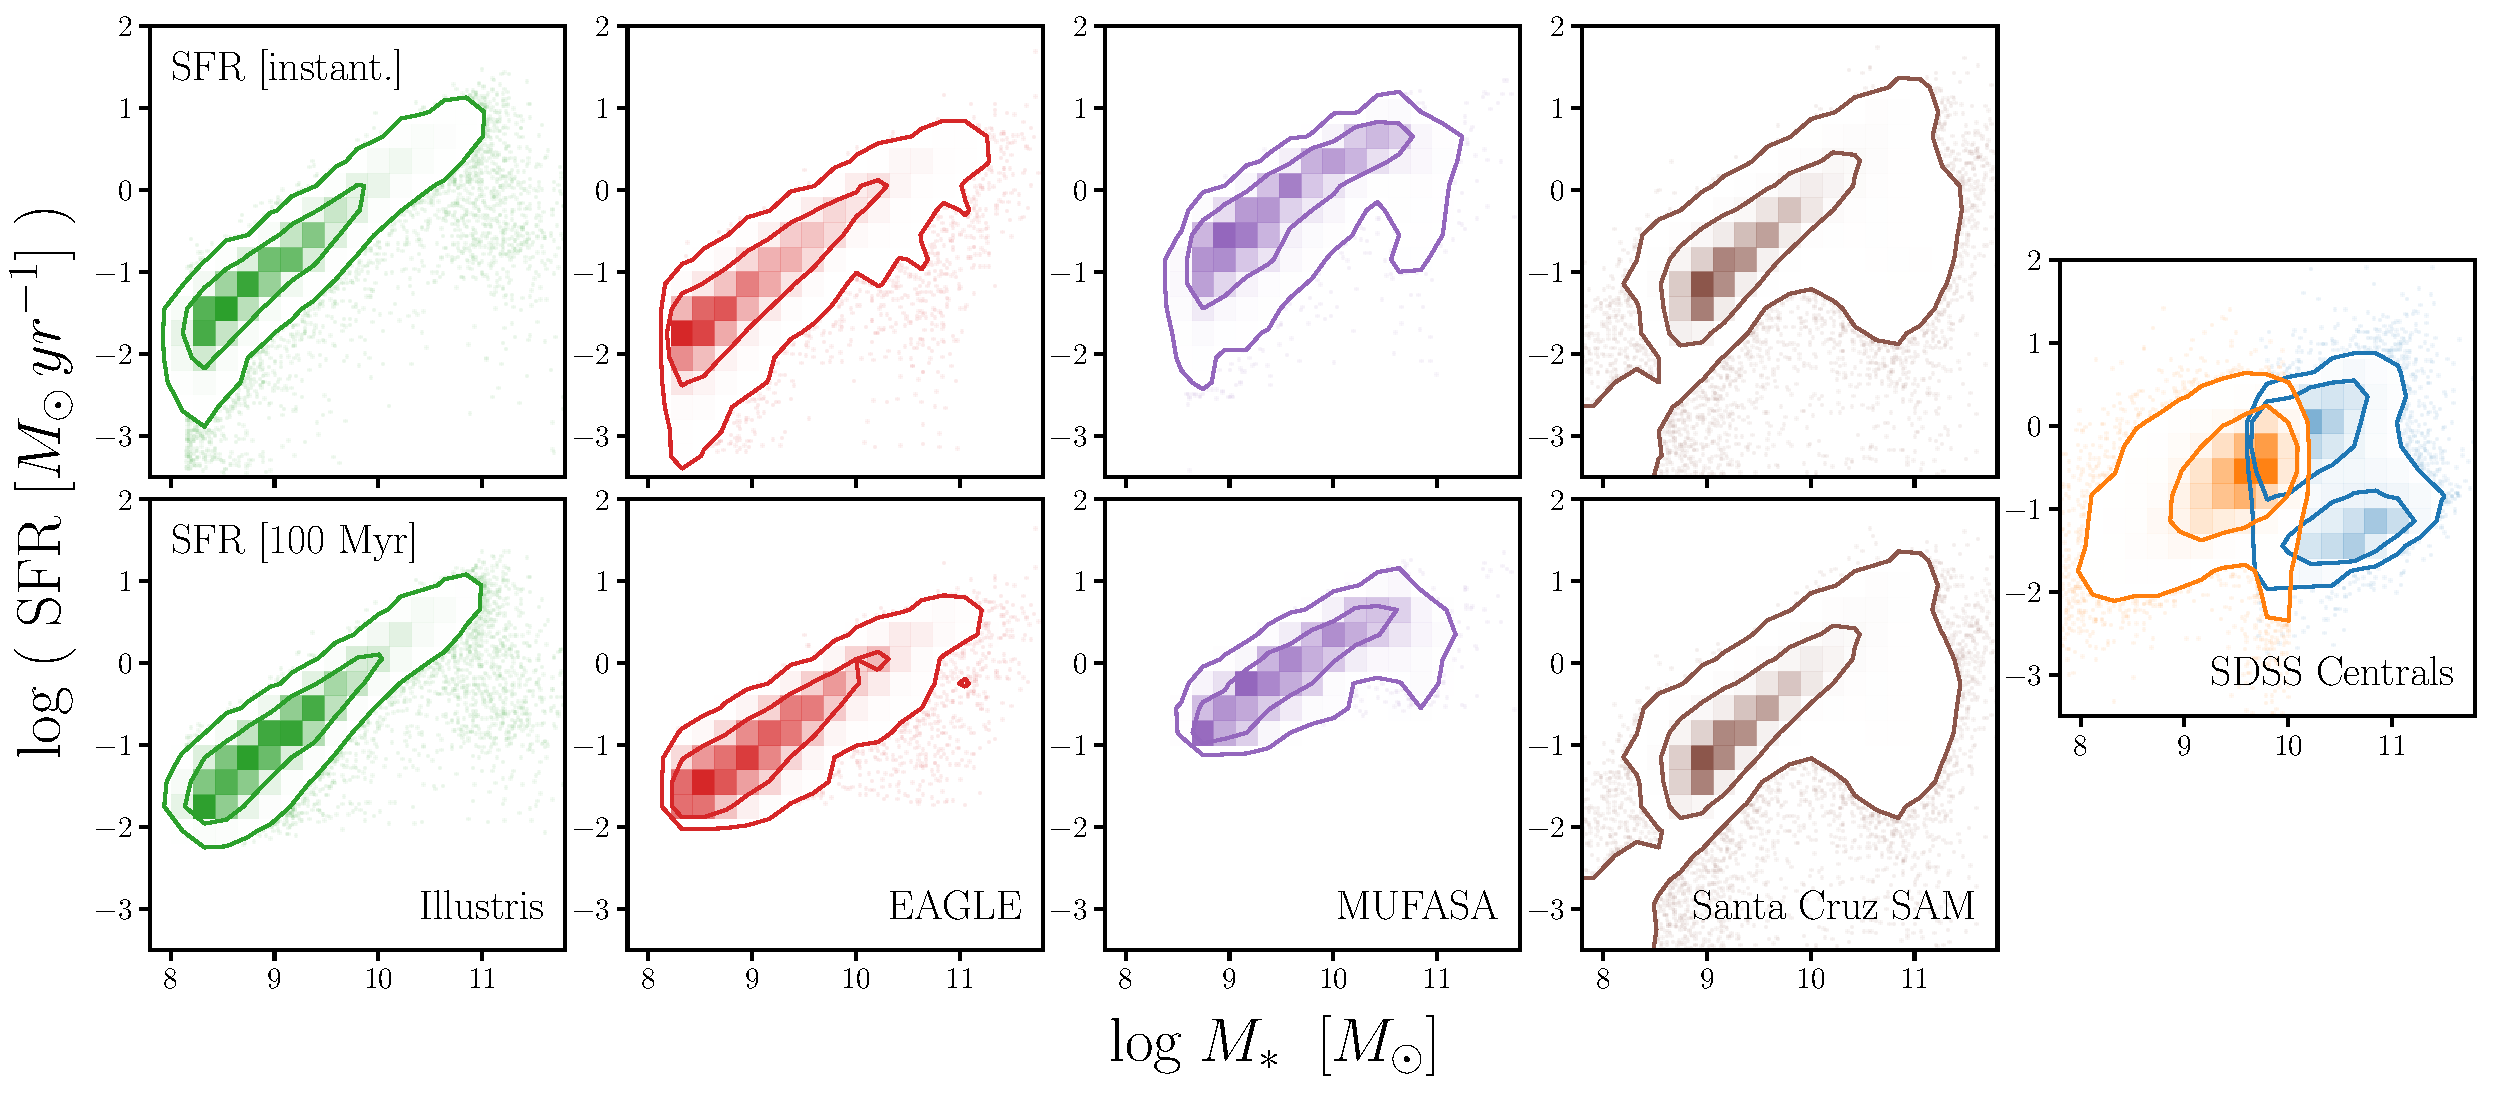
\includegraphics[width=\textwidth]{figs/Catalogs_SFR_Mstar.pdf} 
\caption{The SFR--$M_*$ relations of central galaxies from the Illustris, 
EAGLE, MUFASA, and Santa Cruz SAM simulations (left to right). The 
top panels use instantaneous SFRs while the bottom panels use SFRs 
averaged over $100\,\mathrm{Myr}$. The simulations and how they derive 
the SFRs are described in Section~\ref{sec:galsims}. Although a
direct comparison to observations is tenuous due to the fact that 
the SFRs and $M_*$s of the observed SDSS galaxies are \emph{not} 
derived consistently as simulations, we include, for reference, the 
observed  SDSS galaxies (Section~\ref{sec:obvs}) on the right. 
\emph{The $\mathrm{SFR}--M_*$ relations in every panel reveals a 
clear star forming main sequence.}} 
\label{fig:sfrmstar}
\end{center}
\end{figure*}
%%%%%%%%%%%%%%%%%%%%%%%%%%%%%%%%%%%%%%%%%%

%%%%%%%%%%%%%%%%%%%%%%%%%%%%%%%%%%%%%%%%%%
% Figure  
%%%%%%%%%%%%%%%%%%%%%%%%%%%%%%%%%%%%%%%%%%
\begin{figure}
\begin{center}
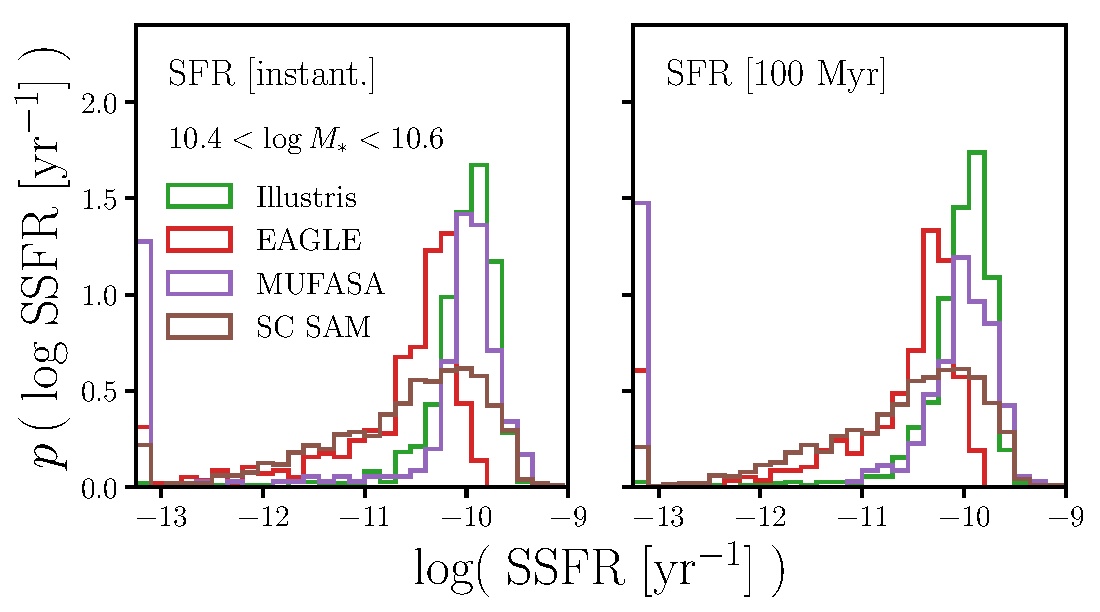
\includegraphics[width=0.475\textwidth]{figs/Catalogs_pSSFR.pdf} 
\caption{The SSFR distributions, $p(\log\,\mathrm{SSFR})$, of the 
central galaxies in the Illustris (green), 
EAGLE (red),  MUFASA (purple), and  Santa Cruz SAM (brown) simulations 
with $10.4 < \log\,M_* < 10.6$. We use instantaneous SFRs on the left
and SFRs averaged over $100\,\mathrm{Myr}$ on the right. Although the
SFMS is universal (Figure~\ref{fig:sfrmstar}), 
\emph{the significant discrepancies among the $p(\log\,\mathrm{SSFR})$s,
and thus SFR--$M_*$ relations, make the SFMS difficult to consistently 
quantify.}} \label{fig:pssfr}
\end{center}
\end{figure}
%%%%%%%%%%%%%%%%%%%%%%%%%%%%%%%%%%%%%%%%%%

\section{Our galaxies} \label{sec:ourgals}
In this work, we primarily focus on simulated galaxy samples from four 
large-scale cosmological simulations: three hydrodynamic (Illustris, EAGLE, 
and MUFASA) and one semi-analytic (Santa Cruz SAM). Although we mainly 
focus on the simulated galaxies, for reference, we also include two observed 
galaxy samples: a volume-limited sample from SDSS and a selected isolated 
dwarf galaxy sample from the NSA catalog. We briefly describe the four 
simulations in Section~\ref{sec:galsims} and our observed galaxy sample 
in Section~\ref{sec:obvs}. %These descriptions primarily focus on the  derivation of SFR's and $M_*$'s in our galaxy samples. 
Lastly in Section~\ref{sec:central}, we describe how we consistently 
identify the central galaxies in both our simulations and observations. 

\subsection{Simulated Galaxies} \label{sec:galsims}
A consistent comparison of the different galaxy populations in our 
simulations requires consistently defined galaxy properties. Hence, 
for all of our simulated galaxies, we derive SFRs consistently on 
two timescales: instantaneous and averaged over $100\,\mathrm{Myr}$. 
Our choice of these timescales is respectively motivated by the fact 
that observed SFR measurements based on $H{\alpha}$ correspond to 
formation of young stars with ages $\lesssim 10\,\mathrm{Myr}$ and 
measurements based on $UV$ brightness correspond to star formation 
in the last $\sim 100\,\mathrm{Myr}$~\citep[e.g.][]{kennicutt2012}. 

%We compare the population of the SFR--$M_{\star}$ plane between the different large-scale cosmological simulations and the observational datasets. To ensure that we compare similar star formation rate timescales, we use averaged star formation rates over chosen recent timescales for all the simulated galaxies. For our analysis, however, we use SFRs averaged 
%over $100\,\mathrm{Myr}$ and instantaneous SFR, to be roughly consistent with respectively observed SFRs based on $H{\alpha}$ observations, corresponding to young stars with ages $\lesssim 10\,\mathrm{Myr}$, and observed SFRs based on $UV$ brightness, corresponding to stars formed in the last $\sim 100\,\mathrm{Myr}$ \citep[e.g.][]{kennicutt2012}. 
More specifically, in our hydrodynamic simulations, we derive the 
$100\,\mathrm{Myr}$ averaged SFRs from the ages, or formation times, 
of star particles in the simulated galaxies and instantaneous SFRs 
from the rate of star formation in the dense and cold gas. For the 
SAM, we derive the $100\,\mathrm{Myr}$ averaged SFRs from the total stellar 
mass formed in a galaxy, which is saved every $10\,\mathrm{Myr}$, and 
the instantaneous SFR based on a Kennicutt-Schmidt relation for 
molecular hydrogen~\citep{bigiel2008} and the derived H$_2$ surface 
density in radial bins.
We note that the spatial \todo{(chang: @tjitske: is spatial correct? Shouldn't the resolution effect be from the mass and time resolution?)} and temporal resolution of our hydrodynamic 
simulation can significantly impact the averaged SFRs. In 
Appendix~\ref{app:zerosfr}, we discuss how we treat
these resolution effects in our analysis.

\todo{chang: How do we derive $M_*$?}

In the rest of this section we provide a brief description of the 
Illustris, EAGLE, MUFASA, and Santa-Cruz SAM simulations and their 
key sub-grid and feedback prescriptions. 

%and how  we derive the instantaneous and $100\,\mathrm{Myr}$ averaged SFRs for  each simulation.

%For the galaxies in the simulations, we compare star formation rates averaged over the last $10\,\mathrm{Myr}$, $100\,\mathrm{Myr}$, and $1\,\mathrm{Gyr}$, as well as the instantaneous SFR. 
%We note that spatial and temporal resolution effects in the simulations  can cause averaged SFRs from stellar ages to under-predict the actual  averaged SFRs in simulations. 
%(most notably the $10\,\mathrm{Myr}$--averaged SFR) can strongly under-predict the actual averaged SFR in the simulations. We therefore add conservative upper limits and uncertainties to these values and study the effect of these on our results.

%Our figures will mostly focus on comparisons of the observationally most relevant timescales (instantaneous, $10\,\mathrm{Myr}$ and $100\,\mathrm{Myr}$) but we will comment on deviations for longer or shorter timescales.


\subsubsection{The Illustris simulation}
The Illustris simulation \citep{vogelsberger2014,genel2014} evolves a
cosmological volume of $(106\ \rm{Mpc})^3$ with a uniform baryonic mass
resolution of $1.6\times10^6M_{\sun}$ using the Arepo moving-mesh code \todo{(chang: citation for code?)}. 
The full halo mass range of $2 \times 10^8$ to $3\times 10^{14}\ M_{\sun}$ 
is set by resolution (32 particles) at the low-mass end and by volume at 
the high-mass end (e.g.~including 10 halos with $M>10^{14}M_{\sun}$). 
It employs sub-grid models for star-formation~\citep{springel2003},
Bondi-like SMBH accretion, a phenomenological model for galactic winds, and 
two main modes for energy injection from 
SMBHs~\citep[\emph{see}][]{vogelsberger2013}. 
When accretion occurs at Eddington ratios $>0.05$, thermal energy is 
injected continuously in the local environment of the SMBH, while at 
lower accretion rates, the energy injection occurs in bursts at large
distances from the SMBH, generating hot bubbles in the ICM~\citep{sijacki2007}.
%The latter mode of feedback is responsible for a steep drop in the  cosmic star-formation rate density at late times~\citep{vogelsberger2013}.
Previous works discussing aspects of the star-formation main-sequence and/or
quenching in the Illustris simulation include 
\citet{vogelsberger2014, sparre2015, bluck2016, terrazas2017}.

\subsubsection{EAGLE}
The Virgo Consortium's Evolution and Assembly of GaLaxies and their 
Environment (EAGLE) project~\citep{schaye2015, crain2015} exists as 
a suite of cosmological, hydrodynamic simulations of a standard 
$\Lambda$ cold dark matter universe using $\mathtt{ANARCHY}$ (Dalla 
Vecchia et al. in prep.; see also Appendix A of \citealt{schaye2015} and 
\citealt{schaller2015}), a modified version of the $\mathtt{Gadget}$ 3 
$N$-body/SPH code ~\citep{springel2005}. 
Modifications include the SPH formulation, time stepping, and subgrid 
physics. The subgrid model for feedback from massive stars and AGN is 
based on thermal energy injection in the ISM without the need to turn-off
cooling or hydrodynamic decoupling of winds~\citep{dallavecchia2012}. 
Similar to SAMs the subgrid parameters for stellar feedback and BH 
accretion are calibrated based on present-day galaxy 
stellar mass function while also requiring reasonable galaxy sizes, and 
the AGN feedback efficiency is constrained by the amplitude of the 
central black hole-galaxy mass relation \todo{(chang: I'm a little confused by this sentence. @tjitske can this be rephrased?)}. 
The simulations resolve galaxies over the stellar mass range 
$10^{8} < M_{\star}/M_{\sun} \lesssim 10^{11}$ and reproduce the galaxy 
stellar mass function to $\lesssim 0.2~\mathrm{dex}$ over this range. 
Of the EAGLE project simulations, we use L0100Ref, which has a volume 
of $(100\,\mathrm{cMpc})^3$ and barynoic mass resolution of 
$1.81\times 10^6M_{\sun}$. The SFR--$M_*$ relation and quenched fractions 
in the EAGLE simulations have been previously discussed 
in~\citet{furlong2015, trayford2015, trayford2017}. 

\subsubsection{MUFASA \todo{[Romeel]}}
\begin{itemize}
	\item \todo{Need to describe the z-dependent halo mass based quenching with continued star formation if self-shielded H2 is present, because we think that causes the turnover in the MUFASA SFMSs.}
\end{itemize}

\subsubsection{the Santa-Cruz Semi-Analytic Model \todo{[Rachel, Viraj]}}

\subsection{Observed SDSS Galaxies} \label{sec:obvs}
\todo{chang: @claire could you check the NSA dwarf galaxy sample description?}
Our main focus in this work is to compare galaxies from our simulation. 
However, since the ultimate goal of the simulations are to reproduce 
observations, we include in our analysis galaxies from the 
SDSS volume-limited sample and the NSA low-luminosity galaxy sample. 
We provide a brief description of the two observed galaxy samples 
below. 

For the SDSS sample, we follow the sample selection of~\cite{tinker2011}. 
We construct the SDSS volume-limited galaxy sample with $M_r - 5\log(h) < -18$ 
and complete in $M_* > 10^{9.7} M_\odot$ from the NYU Value-Added 
Galaxy Catalog \citep[VAGC;][]{blanton2005} which corresponds to 
the SDSS Data Release 7~\citep[DR7;][]{abazajian2009} at redshift 
$z \approx 0.04$. For further details on the sample, we refer readers 
to~\cite{tinker2011,wetzel2013,hahn2017}.

At lower stellar masses, we use an isolated dwarf galaxy sample selected from the NSA catalog as described in \citet{geha2012}. Briefly, the NSA catalog is a reprocessing of SDSS DR8, optimized for low-luminosity 
objects. It relies on the improved background subtraction technique of 
\cite{blanton2011}. The catalog extends to $z \approx 0.055$ and includes 
re-calibrated spectroscopy~\citep{yan2011,yan2012} with much
smaller errors. However, this recalibration is mostly relevant only at small 
equivalent width values and hence galaxies on the star formation main 
sequence will be largely unaffected by this. Dwarf galaxies are considered isolated, and selected, when the distance from a more massive host is $> 1.5 {\rm Mpc}$ \citep{geha2012}.

For both galaxy samples, the stellar masses are estimated using the 
\citet{blanton2007} $\mathtt{kcorrect}$ code, which assumes a 
\cite{chabrier2003} IMF. The SFRs are from the current release 
of~\citet{brinchmann2004}\footnote{http://www.mpa-garching.mpg.de/SDSS/DR7/}, 
where they are derived using the~\cite{bruzuala.1993} model with the 
\cite{charlot2000} dust prescription and CLOUDY \citep[version C90.04;][]{ferland1996} emission line modeling.  
For galaxies classified as having an AGN or a composite spectrum, the 
SFR is measured from the $D_n4000$ index~\citep{balogh1998}. 
Additionally, for starforming galaxies that have low S/N spectra, the SFR 
is derived from the $H{\alpha}$ luminosity~\citep{brinchmann2004}. 
We emphasize that SSFRs $\lesssim 10^{-12} \mathrm{yr}^{-1}$ should only be 
considered upper limits to the true value~\citep{salim2007}.

%are derived following a Bayesian framework where all emission lines are modeled based on the \citet{bruzualCharlot1993, bruzualCharlot1993} galaxy evolution models combined with a dust prescription following \citet{charlotFall2000} and emission line modeling using CLOUDY \citep[version C90.04][]{ferland1996} as described in \citet{charlotLonghetti2001, charlot2002}. 
%For galaxies that are classified as containing an AGN or have a composite (SF and AGN) spectrum, the relation between the derived SFR and Dn4000 index \citep[implemented following][]{Balogh1998} is used to measure the SFR from the Dn4000 index value. Additionally, for galaxies that are starforming but have low S/N spectra the SFR is only dependent on the $H{\alpha}$ luminosity, where the conversion factor used is taken from the distribution function of conversion factors for starforming galaxies with high S/N in the same stellar mass bin \citep{brinchmann2004}. 

%%%%%%%%%%%%%%%%%%%%%%%%%%%%%%%%%%%%%%%%%%%%%%%%%%%%
% Section 
%%%%%%%%%%%%%%%%%%%%%%%%%%%%%%%%%%%%%%%%%%%%%%%%%%%%
\subsection{Identifying Isolated/Central Galaxies} \label{sec:central}
Galaxies and their detailed properties carry the 
imprint of their environment (~\citealt{hubble1936, oemler1974, dressler1980, guzzo1997}, 
for a recent review see~\citealp{blanton2009}). The environment
dependence of, for instance, the quiescent 
fraction~\citep[\emph{e.g.}][]{baldry2006,peng2010,hahn2015}
and the timescale of star formation quenching~\citep{wetzel2013,hahn2017}, 
suggest that different physical mechanisms act in different environments 
to impact galaxy star formation. Also, there may be significant 
discrepancies between the SFMSs of central versus satellite 
galaxies~\citep{wang2018}. Without delving further into the 
environment dependence, \emph{we focus solely on the central galaxies, 
which constitute the majority of massive galaxies ($M_* > 10^{9.5}M_\odot$) 
at $z \sim 0$}. 

Despite its long recognized importance, galaxy environment is often 
heterogeneously defined in the literature~\cite{muldrew2012}. Even among our 
simulations, the classification of centrals depends on 
the definition of halo properties, and thus on the underlying halo 
finders. EAGLE and Illustris use $\mathtt{SUBFIND}$~\citep{springel2001},
where halos are defined as locally overdense, gravitationally bound
(sub)structures within a connected region selected through a 
friend-of-friends~\citep[FOF;][]{davis1985} group finder. On the other hand 
MUFASA and the Santa Cruz SAM are based on halos found using 
$\mathtt{ROCKSTAR}$~\citep{behroozi2013}, which defines halos using a
hierarchical phase-space based FOF technique and endeavors to maximize 
the consistency of the halo through time.  
Regardless of their differences, these central classifications use 
information of the underlying dark matter. Such classifications 
cannot be reproduced on observed galaxy samples and thus complicate 
comparison to observations. Therefore, we identify central galaxies in 
all of our simulations 
consistently using an extended version of the~\cite{tinker2011} group 
finder, designed to identify satellite/centrals in observations. 

%Despite the consistent definition of centrals in the simulations we use, the classification depends on the definition of halo properties in the simulation and thus differences can arise due  to differences in the underlying halo finders used. In the case of our set of simulations both EAGLE and Illustris use
%SUBFIND~\citep{springel2001}, where halos are defined as locally overdense, gravitationally bound (sub)structures within a connected region selected through a friend-of-friends~\citep[FOF]{davis1985} group finder. On the other hand MUFASA and the Santa Cruz SAM are based on halos found using ROCKSTAR~\citep{behroozi2013}, which defines halos using a hierarchical phase-space based FOF technique and endeavors to maximize the consistency of the halo through time. Comparison projects have shown that the halo (central)/subhalo (satellite) classification generally agrees well (although the (sub)halo mass estimation can vary significantly), except when the subhalo is close to the center of the host for example during major mergers, and in late stages of minor mergers~\citep{knebe2011, behroozi2015}. 


\begin{itemize}
    \item \todo{paragraph describing Jeremy's new group finder code} 
\end{itemize}
\emph{Galaxies with $P_\mathrm{sat} < 0.01$ are designated as centrals.} 

Overall, we find good agreement between the central classifications of 
the group finder and simulations. Using purity and completeness as defined 
in Eqs.~13 and~15 of~\cite{campbell2015}, we find central galaxy classification purities of 
$99\%, 93\%, 84\%$, and $90\%$ and completenesses of $86\%$, $89\%$, 
$91\%$, and $86\%$  for the Illustris, EAGLE, MUFASA and Santa Cruz SAM 
simulations respectively. Differences in the purity and completeness for the 
simulations is likely due to the different halo finders used in the 
simulations as described above. For the hydrodynamic simulations, we find no 
significant stellar mass dependence in the purities. However, the Santa 
Cruz SAM has purity of $44\%$ at $M_*$ below $10^{8.5}M_\odot$ and $97\%$ 
above. Consequently, we impose a stellar mass limit of $M_* > 10^{8.5} M_\odot$
for the Santa Cruz SAM. In addition to the overall agreement in central 
classifications, we confirm that the group finder classification does \emph{not} 
impact the results of this paper. In the next section, we proceed to fitting 
the star formation main sequence of simulated galaxies identified as centrals.


%%%%%%%%%%%%%%%%%%%%%%%%%%%%%%%%%%%%%%%%%%
% Figure 
%%%%%%%%%%%%%%%%%%%%%%%%%%%%%%%%%%%%%%%%%%
\begin{figure*}
\begin{center}
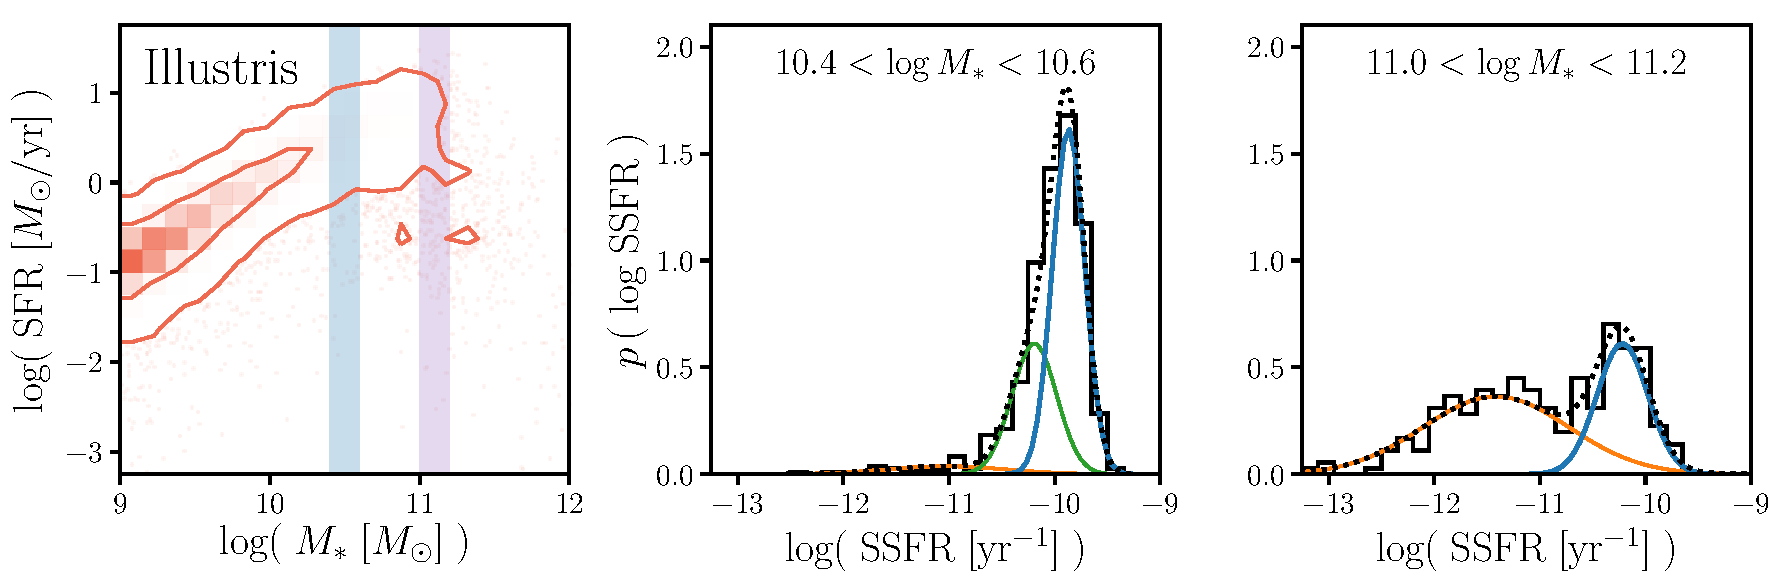
\includegraphics[width = 0.9\textwidth]{figs/SFMSfit_demo.pdf} 
\caption{
We illustrate our GMM SFMS fitting method for Illustris central galaxies in two 
stellar mass bins highlighted on the SFR--$M_*$ relation of the left panel: 
$10.4 < \log\,M_* < 10.6$ and $11.0 < \log\,M_* < 11.2$. On the right, we compare the SSFR 
distributions, $p(\log\,\mathrm{SSFR})$, in the two stellar 
mass bins to their best-fit GMMs. The $p(\log\,\mathrm{SSFR})$ in the center panel is best described by a 
GMM with three components (orange, green, and blue) while the
$p(\log\,\mathrm{SSFR})$ in the right panel is best described by 
a GMM with two components (orange and blue). The SFMS components of the 
best-fit GMMs are plotted in blue. \emph{Our GMM SFMS fitting provides
a flexible and data-driven way to identify the SFMS for a wide variety 
of SSFR distributions without hard assumptions or cuts to the sample.}
}\label{fig:fitdemo}
\end{center}
\end{figure*}
%%%%%%%%%%%%%%%%%%%%%%%%%%%%%%%%%%%%%%%%%%

\section{Fitting the Star Formation Main Sequence}\label{sec:sfmsfit}
We present the SFR--$M_*$ relation of central galaxies identified 
from the simulations and observations of Section~\ref{sec:ourgals} in 
Figure~\ref{fig:sfrmstar}. Regardless of SFR timescale (top/bottom),
for both simulations and observations, and over four orders of magnitude 
in stellar mass, \emph{the SFR and $M_*$ of star-forming galaxies lie 
tightly correlated on the SFMS}. A well-defined SFMS can be found in 
each panel of Figure~\ref{fig:sfrmstar}.

Despite its universality among multiple observations and simulations, 
different datasets give rise to significantly SFR--$M_*$ distributions.
This makes the SFMS difficult to \emph{consistently} quantify. So far 
in the literature, a wide variety 
of fitting methods have been applied to data. For instance, \cite{bluck2016} 
fit the SFMS using median $\log\mathrm{SFR}$s of galaxies with 
$M_* < 10^{10}M_\odot$ and extrapolate to higher masses. This method, however, 
assumes that all $M_* < 10^{10}M_\odot$ galaxies lie on the SFMS and that 
there is no variation in the slope of the SFMS at higher stellar masses. 
Alternatively, \cite{lee2015} fit the SFMS using median 
$\log\,\mathrm{SFR}$s of galaxies in the sample after some color-color cut 
to identify SF galaxies. Other recent works in the literature have opted 
for more sophisticated methods such as fitting a three-component
Gaussian~\citep{bisigello2018} or a zero-inflated negative binomial 
distribution~\citep{feldmann2017}. 

All of these methods require arbitrary assumptions or hard cuts on the 
sample. Moreover, these methods struggle with fitting the SFMS over a 
wide SFR or $M_*$ range and for the wide variety of SSFR distributions we see 
in simulations and observations. Even for fixed a stellar mass bin 
($10.4 < \log M_* < 10.6$), Figure~\ref{fig:pssfr} reveals the 
significant discrepancies in the SSFR distributions of our four simulations. 
Therefore, in an effort to better fit a wide variety of star formation--stellar
mass distributions and to relax the assumptions and cuts imposed on the data, 
\emph{we present a flexible and data-driven method for fitting the SFMS that 
makes use of Gaussian Mixture 
Models}~\citep[][]{Press:1992:NRC:148286, 9780471006268}. 

\subsection{Using Gaussian Mixture Models}
Gaussian mixture models (hereafter GMM), and mixture models in general, provide 
a probabilistic way of describing the distribution of a population by 
identifying subpopulations from the data. Besides their extensive use 
in machine learning and statistics, GMMs has also been used in wide range 
of astronomical analyses~\citep{bovy2011,lee2012,taylor2015}. 
Since identifying the subpopulation of star forming galaxies from the overall
galaxy population is equivalent to fitting the SFMS, GMMs provides a 
well-motivated, data-driven, and effective method to tackle the problem. 

A GMM, more precisely, is a weighted sum of $k$ Gaussian component densities 
\begin{equation} \label{eq:gmm}
\hat{p}(x;\bm{\theta}) = \sum\limits_{i=1}^{k} \pi_i \, \mathcal{N}(x; \bm{\theta}_i),
\end{equation}
to estimate the density. The weights, $\pi_i$, mean, and variance  
$\bm{\theta}_i=\{\mu_i, \sigma_i\}$ 
of the components are free parameters in the GMM. For a given data set 
$\{x_1, ..., x_n\}$, these parameters are most commonly estimated through
the expectation-maximization algorithm~\citep[EM;]{dempster1977,neal1998}. 

Starting with randomly assigned $\bm{\theta}_{i}^0$ to the $k$ GMM components, 
the EM algorithm iterates between two steps. First, for every data point, 
$x_i$, the algorithm computes for a probability of $x_i$ being generated by 
each GMM component. These probabilities act as assignment weights to each of
the components. Next, based on these weights, $\bm{\theta}_i^t$ of the components 
are updated to $\bm{\theta}_i^{t+1}$ to maximize the likelihood of the assigned 
data. $\pi_i$ are also updated by summing up the assignment weights and 
normalizing the sum by the total number of data points. These steps are 
repeated until convergence --- \emph{i.e.} when $p(\{x_1, ..., x_n\} ; \bm{\theta}_t)$ 
converges. Instead of starting with randomly assigning $\bm{\theta}_{i}^0$, 
we initiate our EM algorithm using a $k$-means clustering algorithm~\citep{lloyd1982}.
More specifically, for our Gaussian mixture density estimation we use 
the $k$-$\mathtt{means}$++ algorithm of~\cite{arthur2007}. 

For our actual SFMS fitting method, we first divide the galaxy 
sample into stellar mass bins of width $\Delta \log\,M∗$. In 
this paper we use bins of $\Delta \log\,M∗ = 0.2\  \mathrm{dex}$; however, 
this choice does not significantly impact the final fit. For each stellar 
mass bin, if there are more than $N_\mathrm{thresh}=100$ galaxies in the bin, 
we fit the SSFR distribution using Gaussian mixture models (GMMs) 
with 1 to 3 components with parameters determined from the EM algorithm 
described above. Our restriction to models with a maximum of 3 components 
is motivated by the three main galaxy classifications: quiescent, 
star-forming, and transitioning populations. Furthermore, for our observed 
galaxy samples, even when we allow for more than 3 components, 
the best-fit GMMs have $k\leq3$. We confirm that restricting ourselves 
to 3 components does not significantly impact the results of this work
(Appendix~\ref{app:gmm}). 

Out of the three ($k\leq3$) GMMs, we select the ``best-fit'' model with the lowest Bayesian Information 
Criteria~\citep[BIC;][]{schwarz1978}. BIC is often used in conjunction with 
GMMs~\citep[\emph{e.g.}][]{leroux1992,roeder1997,fraley1998,steele2010performance} 
and also more generally for model selection in 
astronomy~\citep[\emph{e.g.}][]{liddle2007,broderick2011,vakili2016}.
In addition to the likelihood, BIC introduces a penalty term for the number
of parameters in the model. This way, using BIC not only finds a good fit to 
the data, but it also addresses the concern of over-fitting. 
% CHH: not sure if we want to include this figure}.
% In Figure~\ref{fig:gmm_pedagog},  

In the best-fit GMM, we designate the Gaussian component of the 
best-fit GMM with mean $\log\,\mathrm{SSFR} > −11$ as the SFMS component.
In the case when more than one GMM component has mean 
$\log\,\mathrm{SSFR} > −11$, the component with the larger weight 
(\emph{i.e.} the mode) is designated as the SFMS component. Typically in such a 
situation, the SFRs of the SFMS is not well described by a log-normal
distribution. In observations, we do not encounter this situation. 
In simulations, however, we encounter this situation in lower stellar mass bins 
($\log\,M_* < 10^{9}\ M_\odot$) of the Illustris and EAGLE simulations. 

In Figure~\ref{fig:fitdemo}, we illustrate our GMM SFMS fitting for the 
central galaxies of the Illustris simulation in two stellar mass 
ranges highlighted in the left panel: $10.4 < \log\,M_* < 10.6$ (center) 
and $11.0 < \log\,M_* < 11.2$ (right). For the two stellar mass bins, 
we compare the SSFR distributions of the bins to the components of the 
best-fit GMMs derived from our SFMS fitting method. The SFMS component 
is plotted in blue. The SSFR distribution of the center panel is best 
described by a GMM with three components while the SSFR distribution 
in the right  panel is best described by a GMM with only two components.
%The right panels illustrate the wide variation in SSFR distributions of the galaxy samples. 
These comparisons highlights the flexibility and effectiveness 
of our fitting method in identifying the SFMS for different SSFR 
distributions. All the code used for our SFMS fitting is publicly available 
at \url{https://github.com/changhoonhahn/LetsTalkAboutQuench}.

%%%%%%%%%%%%%%%%%%%%%%%%%%%%%%%%%%%%%%%%%%
% Figure
%%%%%%%%%%%%%%%%%%%%%%%%%%%%%%%%%%%%%%%%%%
\begin{figure*}
\begin{center}
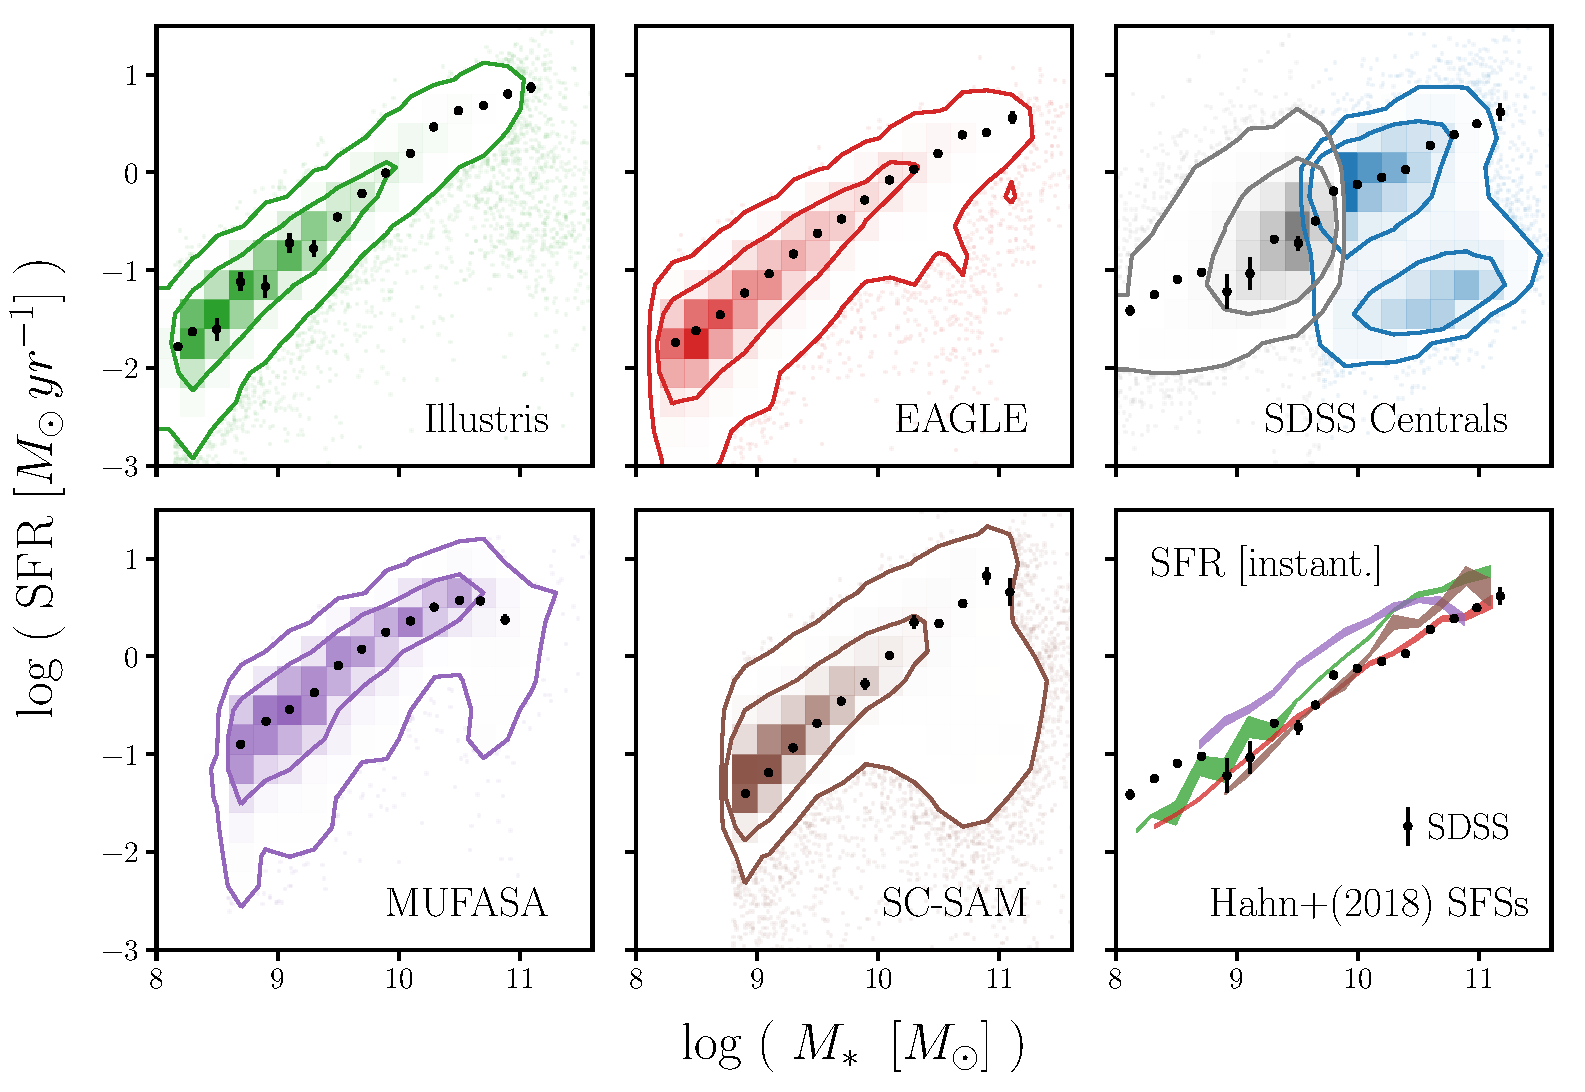
\includegraphics[width = 0.8\textwidth]{figs/Catalogs_SFMSfit_SFRinst.pdf} 
\caption{Best-fit SFMS of the central galaxies in the Illustris, EAGLE, MUFASA, 
    and Santa Cruz SAM simulations as identified by our SFMS GMM fitting method 
    (Section~\ref{sec:sfmsfit}). The SFMSs above are fit from the instantaneous 
    SFR--$M_*$ relation. For reference, we include the best-fit SFMS of the SDSS 
    sample in the top right panel. The uncertainties of the best-fit SFMS are
    derived usig bootstrap resampling. When we compare the SFMS fits
    (bottom right panel), \emph{the SFMSs of the simulations have similar 
    overall stellar mass dependence, but their amplitude vary roughly by an 
    order of magnitude.}} \label{fig:sfmsfit_inst}
\end{center}
\end{figure*}
%%%%%%%%%%%%%%%%%%%%%%%%%%%%%%%%%%%%%%%%%%

%%%%%%%%%%%%%%%%%%%%%%%%%%%%%%%%%%%%%%%%%%
% Figure  
%%%%%%%%%%%%%%%%%%%%%%%%%%%%%%%%%%%%%%%%%%
\begin{figure*}
\begin{center}
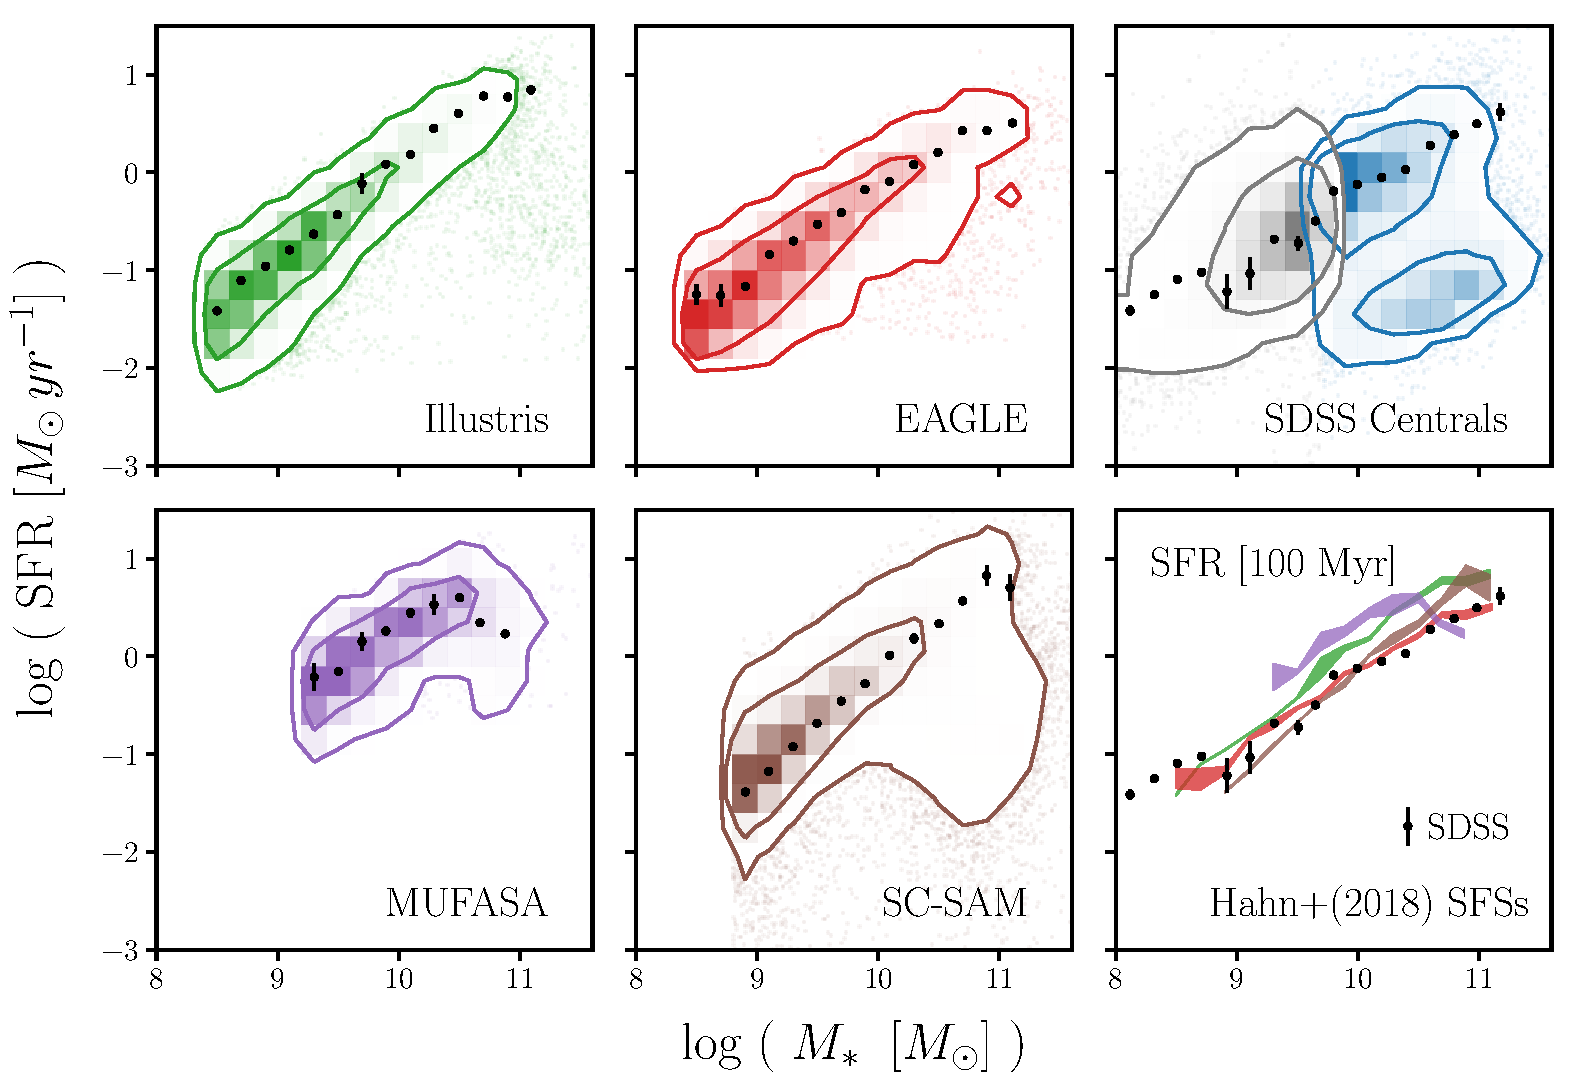
\includegraphics[width = 0.8\textwidth]{figs/Catalogs_SFMSfit_SFR100myr.pdf} 
    \caption{Same as Figure~\ref{fig:sfmsfit_inst} but for the $100\,\mathrm{Myr}$ 
    SFR--$M_*$ relation. As in Figure~\ref{fig:sfmsfit_inst}, \emph{the SFMSs of the simulations have 
    similar stellar mass dependence but vary roughly by an order of magnitude in amplitude.}}
\label{fig:sfmsfit_100myr}
\end{center}
\end{figure*}
%%%%%%%%%%%%%%%%%%%%%%%%%%%%%%%%%%%%%%%%%%

%%%%%%%%%%%%%%%%%%%%%%%%%%%%%%%%%%%%%%%%%%
% Figure  
%%%%%%%%%%%%%%%%%%%%%%%%%%%%%%%%%%%%%%%%%%
\begin{figure}
\begin{center}
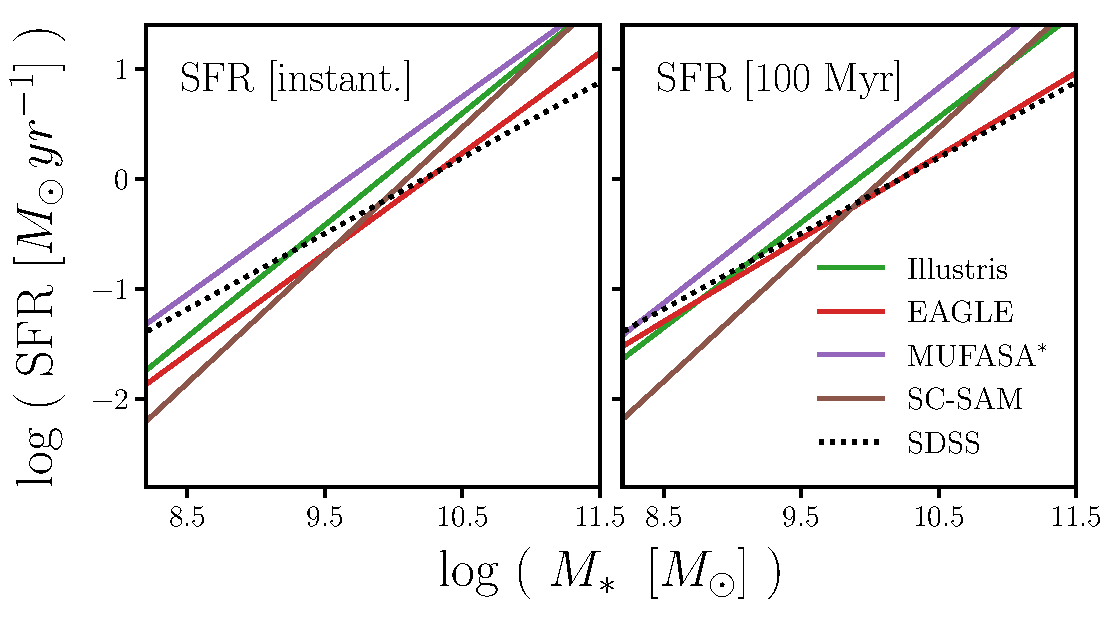
\includegraphics[width = 0.5\textwidth]{figs/Catalogs_SFMS_powerlawfit.pdf} 
\caption{Power-law fits to the best-fit SFMS for the Illustris (green), 
    EAGLE (red), MUFASA (purple), and Santa Cruz SAM (brown) simulations. 
    The left and right panels use instantaneous SFR and $100\,\mathrm{Myr}$ 
    SFR, respectively. We list the power-law fit parameters in 
    Table~\ref{tab:sfms_powerlaw}. The power-law fit to the MUFASA SFMS 
    is impacted by the high stellar mass turnover. The power-law fits for 
    the Illustris, EAGLE, and Santa Cruz SAM SFMS differ by \todo{${\sim}0.5\,\mathrm{dex}$}
    with no significant mass dependence.}
    \label{fig:sfmsfit_powerlaw}
\end{center}
\end{figure}
%%%%%%%%%%%%%%%%%%%%%%%%%%%%%%%%%%%%%%%%%%

\section{Results} \label{sec:results}
\subsection{SFMS of simulated galaxies}
Now with our method for fitting the SFMS, which can be flexibly 
applied a wide range of SSFR distributions, we identify the SFMSs of our simulated
central galaxies from Section~\ref{sec:ourgals}. For the instantaneous and 
$100\,\mathrm{Myr}$ SFR timescales, we present the best-fit SFMSs of our 
simulated galaxies from the Illustris, EAGLE, MUFASA, and Santa Cruz SAM 
simulations in Figures~\ref{fig:sfmsfit_inst} and~\ref{fig:sfmsfit_100myr}, 
respectively. %For reference we include the best-fit SFMS of the SDSS central galaxies in the top right panel. 

The best-fit SFMSs of the Illustris, EAGLE, and Santa Cruz SAM simulations
exhibit a similar monotonic relation between SFR and $M_*$ out to 
$M_* \gtrsim 10^{11}M_\odot$, for both SFR timescales. The best-fit SFMSs 
for MUFASA, however, turn over at 
$M_*{\sim}10^{10.5} M_\odot$ and decreases in SFR at high stellar masses. 
We confirm that this turnover is \emph{not} caused by misidentification of 
the SFMS or some systematic effect of the fitting by examining the 
best-fit GMM components  and the $p(\log\mathrm{SSFR})$ in these higher 
stellar mass bins. Between the two SFR timescales, we find little difference 
between the best-fit SFMSs for each simulation. However, when we compare the 
best-fit SFMSs of the simulations altogether in more detail, we find 
\emph{order of magnitude discrepancies in SFR among the best-fits throughout 
the stellar mass range of the simulations for both SFR timescales} (bottom 
right panels of Figures~\ref{fig:sfmsfit_inst} and~\ref{fig:sfmsfit_100myr}). 
%These best-fit SFMSs allow us to make detailed comparison among the simulations. 

The uncertainties for the best-fit SFMSs in Figures~\ref{fig:sfmsfit_inst} 
and~\ref{fig:sfmsfit_100myr} are derived from bootstrap resampling~\citep{efron1979} 
in each stellar mass bin of the fitting. These uncertainties are \emph{underestimates} because 
they do not account for ``cosmic variance'' --- \emph{i.e.} we only have one 
finite volume realization of each simulation. Furthermore, uncertainty of the best-fit 
SFMS corresponds to the uncertainty of the means of the SFMS GMM component, 
which is only one of the parameters in the GMM. Uncertainties from bootstrap 
resampling, however, do \emph{not} account for the correlations between the 
mean of the SFMS GMM and other
parameters of the GMM (Eq.~\ref{eq:gmm}). A more robust estimate of the 
uncertainties would involve estimating the marginalized posterior distribution 
of the SFMS GMM component mean using a method like MCMC. Since this still 
does not account for cosmic variance, we use bootstrap uncertainties. 

From the best-fit SFMSs, we can further 
parameterize the SFMS to some functional form as often done in the 
literature --- \emph{e.g.} power-law~\citep{speagle2014} or broken 
power-law~\citep{lee2015}. With little evidence of a turnover in the 
SFMS for most of our galaxies, we fit a power-law of the form 
\begin{equation} \label{eq:powerlaw}
\log\,\mathrm{SFR}_\mathrm{MS} = m\,(\log\,M_* - 10.5) + b
\end{equation}
to the SFMSs in Figure~\ref{fig:sfmsfit_powerlaw}. We list the best-fit 
(maximum likelihood) parameter values of Eq.~\ref{eq:powerlaw} in 
Table~\ref{tab:sfms_powerlaw}. The power-law parameterizations accentuate 
the stellar mass dependence of the SFMSs and can reveal the mass dependence 
in the SFMS discrepancies. Putting aside MUFASA, whose power-law fit is 
impacted by the turnover at high stellar masses, we find significant
discrepancies in the slopes of the SFMSs of the simulations with Santa Cruz 
SAM having the steepest SFMS and EAGLE having the shallowest SFMS. The 
power-law SFMS fits, however, reveal little 
mass dependence in the discrepancies of the SFMSs. For instantaneous SFR, 
the discrepancies between the SFMSs of Illustris, EAGLE, and Santa Cruz SAM are 
$\sim 0.5\,\mathrm{dex}$ throughout the stellar mass range. Meanwhile, 
for $100\,\mathrm{Myr}$ SFR, we find slightly
greater discrepancies among Illustris, EAGLE, and Santa Cruz SAM throughout
the stellar mass range.

%At lower stellar masses (), for both instantaneous SFRs and $100\,\mathrm{Myr}$ SFRs, the SFMS disagree with each  other by more than an order of magnitude. \todo{talk about how MUFASA for 100 Myr is an outlier because of the high  stellar mass limit and the high mass turnover.}
Things to discuss at the workshop: 
\begin{itemize}
\item \todo{What's causing the simulations to have SFMSs that are almost an 
order of magnitude different?} 
\item \todo{How come this doesn't cause cosmic star-formation rate 
density estimates to also be an order of magnitude different? Is it that they agree better on the total or average SFR in a stellar mass bin than on how we model the SFMS??}
\item \todo{what's up with MUFASA. why does MUFASA have a turnover? -- 
Due to MUFASA's quenching method being based on halo mass?}
\end{itemize}

In addition to its position, $\mu_\mathrm{SFMS}$, the SFMS GMM component 
is also described by $\sigma_\mathrm{SFMS}$ --- the width of the SFMS. 
Using $\sigma_\mathrm{SFMS}$ derived from the SFMS GMM fitting, 
we can compare the width of the SFMS among the simluations 
(Figure~\ref{fig:sfms_width}). The uncertainties for the widths are 
calculated through bootstrap resampling in the same way as the 
uncertainties for the SFMS fits. Overall, we find little stellar mass 
dependence in $\sigma_\mathrm{SFMS}$ for the simulations. For Illustris, 
EAGLE, MUFASA, and Santa Cruz SAM we respectively find 
$\sigma_\mathrm{SFMS} \sim 0.16, 0.20, 0.21$, and $0.20\,\mathrm{dex}$ 
for instantaneous SFR and
$\sigma_\mathrm{SFMS} \sim 0.17, 0.24, 0.23$, and $0.24\,\mathrm{dex}$
for $100\,\mathrm{Myr}$ SFR. These $\sigma_\mathrm{SFMS}$ are narrower 
than the ${\sim}0.3\,\mathrm{dex}$ width measured in 
observations~\citep[\emph{e.g.}][]{daddi2007, noeske2007, magdis2012, whitaker2012}. 
This difference, however, does not account for the uncertainties in the 
observed SFR measurements, which would reduce the discrepancy. We 
therefore conclude that \emph{the width of the SFMS from our 
simulations are in agreement with the observed SFMS width.}


%%%%%%%%%%%%%%%%%%%%%%%%%%%%%%%%%%%%%%%%%%
% Table
%%%%%%%%%%%%%%%%%%%%%%%%%%%%%%%%%%%%%%%%%%
\begin{table}
\caption{Power-law fit to the SFMS of our simulated central galaxies from the
Illustris, EAGLE, MUFASA, and Santa Cruz SAM simulations.\todo{update}} 
\begin{center}
\begin{tabular}{p{5cm}cc} \toprule
%\multicolumn{2}{c}{} \\[-7pt]
\multicolumn{3}{c}{Star Forming Main Sequence fit} \\
\multicolumn{3}{c}{$\log\,\mathrm{SFR}_\mathrm{MS} = m\,(\log\,M_* - 10.5) + b$  } \\ [5pt]
Simulation & $m$ & $b$ \\ 
\hline
Illustris [inst. SFR] & 0.96 & 0.51 \\ 
Illustris [$100\,\mathrm{Myr}$ SFR] & 0.96 & 0.54 \\ [2pt]
EAGLE [inst. SFR] & 0.86 & 0.17 \\ 
EAGLE [$100\,\mathrm{Myr}$ SFR] & 0.76 & 0.18 \\ [2pt]
MUFASA [inst. SFR] & 0.69 & 0.50 \\ 
MUFASA [$100\,\mathrm{Myr}$ SFR] & 0.57 & 0.44 \\ [2pt]
Santa Cruz SAM [inst. SFR] & 1.10 & 0.36 \\ 
Santa Cruz SAM [$100\,\mathrm{Myr}$ SFR] & 1.11 & 0.36 \\ 
\hline
\end{tabular} \label{tab:sfms_powerlaw}
\end{center}
\end{table}
%%%%%%%%%%%%%%%%%%%%%%%%%%%%%%%%%%%%%%%%%%

One factor that impacts our SFMS fits is the strict lower limit of the 
$\log\mathrm{SFR}$s caused by the resolution effects in the simulations. 
This is particularly evident in the $100\,\mathrm{Myr}$ SFR--$M_*$ 
relations of the hydrodynamic simulations of Figure~\ref{fig:sfrmstar}---especially 
MUFASA. As we describe in Section~\ref{sec:galsims}, the $100\,\mathrm{Myr}$ 
SFRs are  calculated using the ages of all star particles in a galaxy. For a galaxy to 
have star formation (\emph{i.e.} SFR $> 0$), it must \emph{at least} 
form one star particle over the last $100\,\mathrm{Myr}$. A single star particle 
forming over $100\,\mathrm{Myr}$ amounts to a SFR of 
$\sim 0.02\ M_{\sun}\ yr^{-1}$ for Illustris and EAGLE and
$\sim 0.2\ M_{\sun}\ yr^{-1}$ for MUFASA. This resolution limit, ultimately 
impacts the SFMS fits at stellar masses below $10^{8.4}$, $10^{8.6}$, and 
$10^{9.4}M_\odot$ for Illustris, EAGLE, and MUFASA respectively. 
These stellar mass limits have accordingly been imposed on the SFMS fits
and power-law SFMS fits in Figures~\ref{fig:sfmsfit_100myr} 
and~\ref{fig:sfmsfit_powerlaw}. In Appendix~\ref{app:zerosfr}, we describe
how we derive these stellar mass limits. 

By using the SFMS fitting method we present in this paper, we're able to 
conduct a principled data-driven comparison of the SFMSs of central galaxies 
from the Illustris, EAGLE, MUFASA, and Santa Cruz SAM simulations. From 
this comparison, we find that the amplitudes of the SFMSs differ from one 
another by an order of magnitude, with no significant stellar mass dependence. 
Furthermore, despite the discrepancies in their amplitude, the SFMSs of 
our simulations have similar widths, consistent with observations. 
%%%%%%%%%%%%%%%%%%%%%%%%%%%%%%%%%%%%%%%%%%
% Figure  
%%%%%%%%%%%%%%%%%%%%%%%%%%%%%%%%%%%%%%%%%%
\begin{figure}
\begin{center}
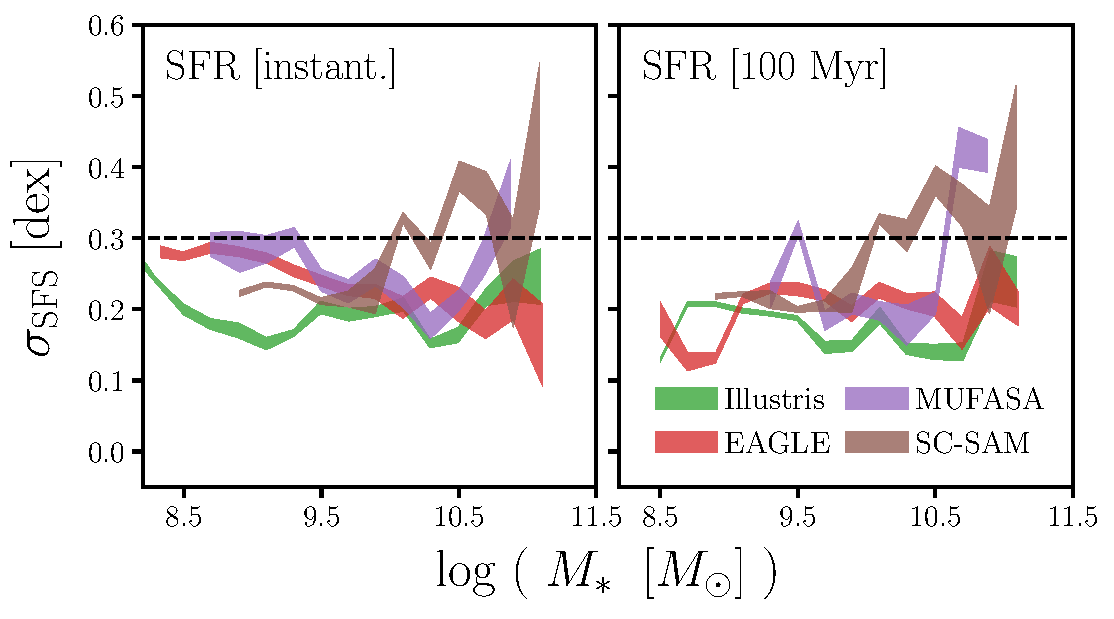
\includegraphics[width=0.48\textwidth]{figs/Catalogs_SFMS_width.pdf}
\caption{The width of the SFMS, $\sigma_\mathrm{SFMS}$, for our simulated 
    central galaxies from Illustris, EAGLE, MUFASA, and Santa Cruz SAM 
    (green, red, purple, and brown respectively). The widths are derived from  
    the GMM SFMS fitting and its uncertainties are estimated using bootstrap
    resampling in the same way as the SFMS fit uncertainties. 
    $\sigma_\mathrm{SFMS}$s in our simulations have little stellar mass 
    dependence and, naively accounting for measurement errors in observed 
    SFR, they are consistent with $\sigma_\mathrm{SFMS}{\sim}0.3\,\mathrm{dex}$ 
    from observations (black dashed).} \label{fig:sfms_width}
\end{center}
\end{figure}
%%%%%%%%%%%%%%%%%%%%%%%%%%%%%%%%%%%%%%%%%%


%%%%%%%%%%%%%%%%%%%%%%%%%%%%%%%%%%%%%%%%%%
% Figure  
%%%%%%%%%%%%%%%%%%%%%%%%%%%%%%%%%%%%%%%%%%
\begin{figure*}
\begin{center}
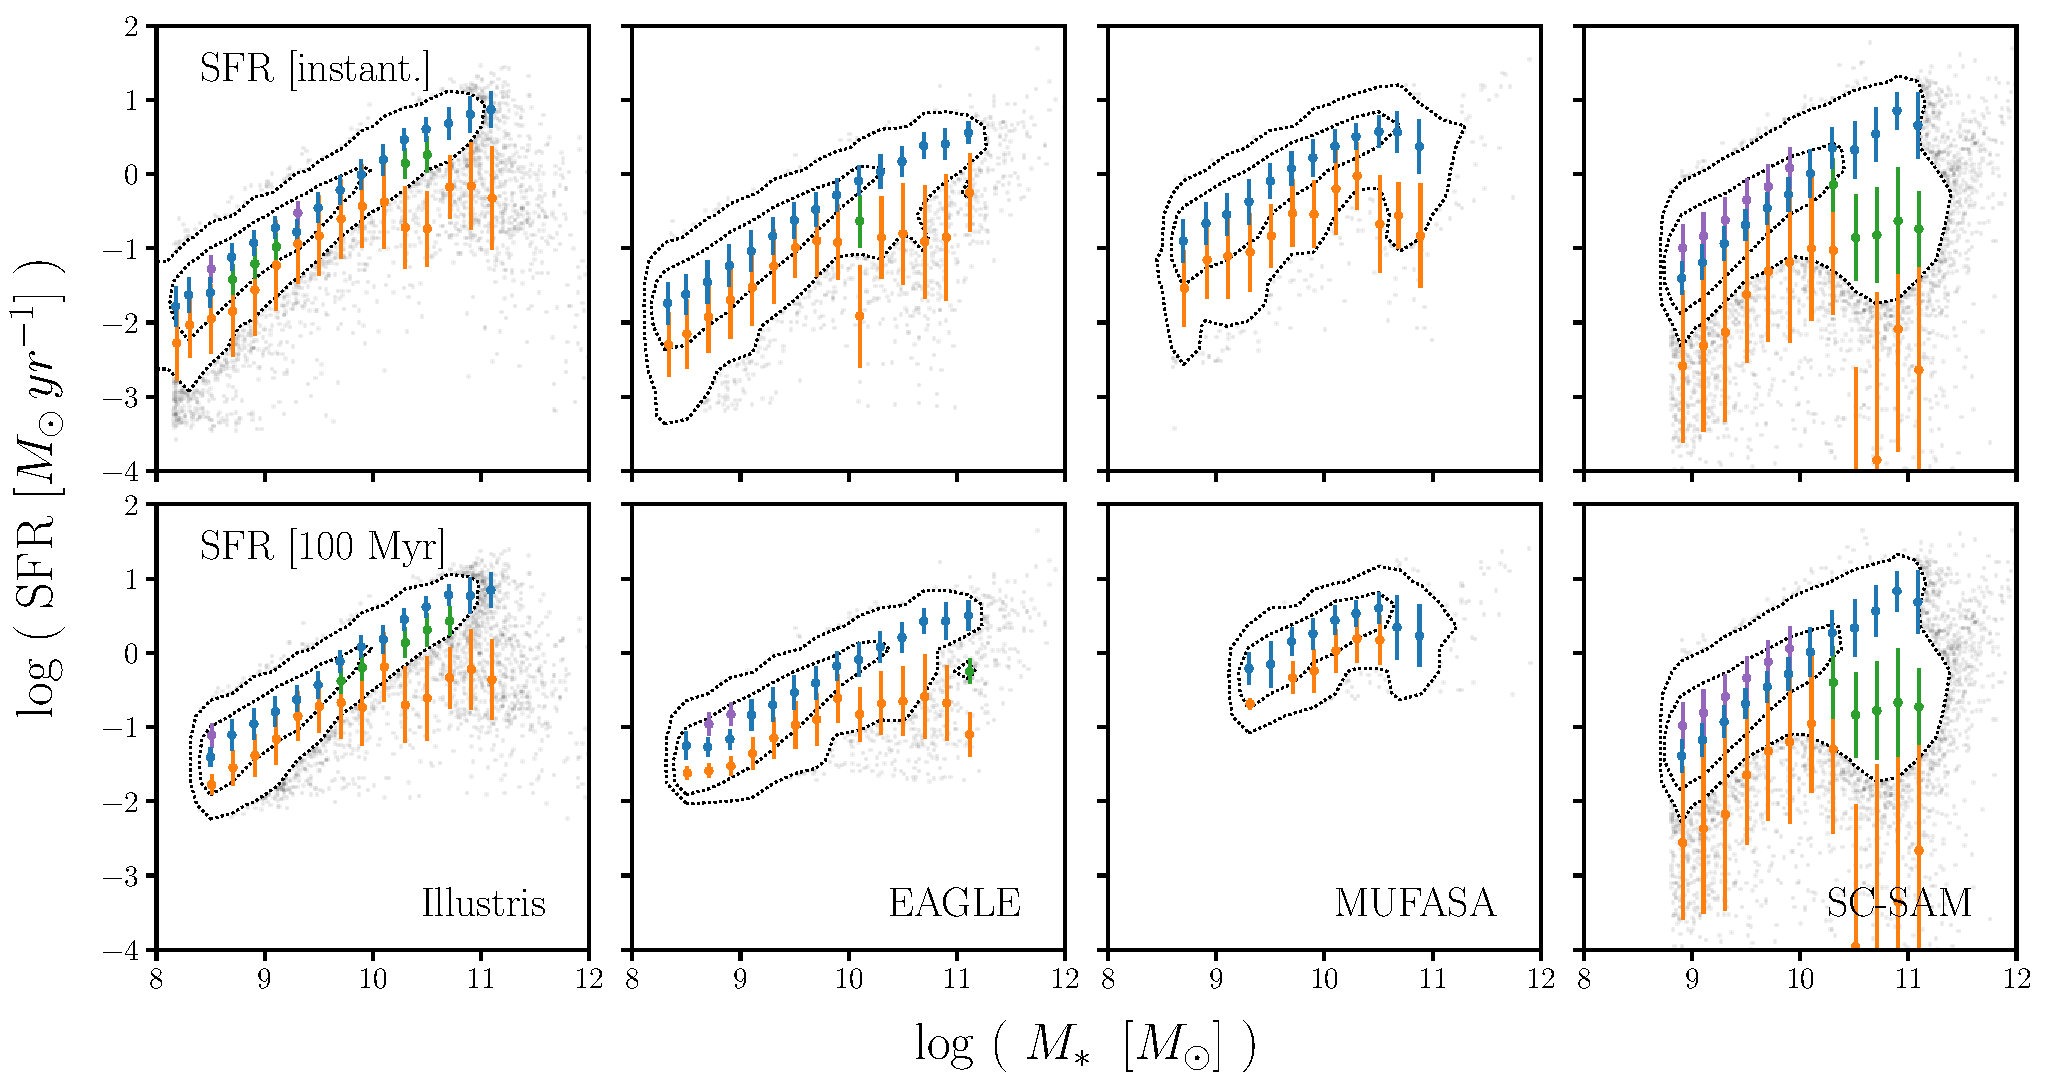
\includegraphics[width=\textwidth]{figs/Catalogs_GMMcomps.pdf} 
\caption{Components of the best-fit GMM from our SFMS fitting method for the
    SFR-$M_*$ relations of central galaxies in the Illustris, EAGLE, MUFASA, and 
    Santa Cruz SAM simulations (left to right). The top panels use instantaneous 
    SFRs while the bottom panels use SFRs averaged over $100\,\mathrm{Myr}$.  %For reference, we also include observed centrals from SDSS (top right). 
    We mark the SFMS components in blue, the components with lowest SFR in orange, 
    and the other components in green. These components roughly correspond to the 
    star-forming, quiescent, and transitioning or star-burst populations. 
    Among the hydrodynamical simulations, despite the SFMS discrepancies,
    (Figures~\ref{fig:sfmsfit_inst} and~\ref{fig:sfmsfit_100myr}), the GMM components 
    reveal overall similarities in the galaxy populations. Meanwhile for the Santa Cruz 
    SAM, the GMM components reveal its broad quenched component that extends beyond 
    $\mathrm{SFR} < 10^{-4}M_\odot yr^{-1}$ and prominent transitioning components at 
    $M_* > 10^{10}M_\odot$, different from the hydrodynamic simulations. 
    } \label{fig:sfmsfit_comps}
\end{center}
\end{figure*}
%%%%%%%%%%%%%%%%%%%%%%%%%%%%%%%%%%%%%%%%%%


%%%%%%%%%%%%%%%%%%%%%%%%%%%%%%%%%%%%%%%%%%
% Figure 
%%%%%%%%%%%%%%%%%%%%%%%%%%%%%%%%%%%%%%%%%%
\begin{figure*}
\begin{center}
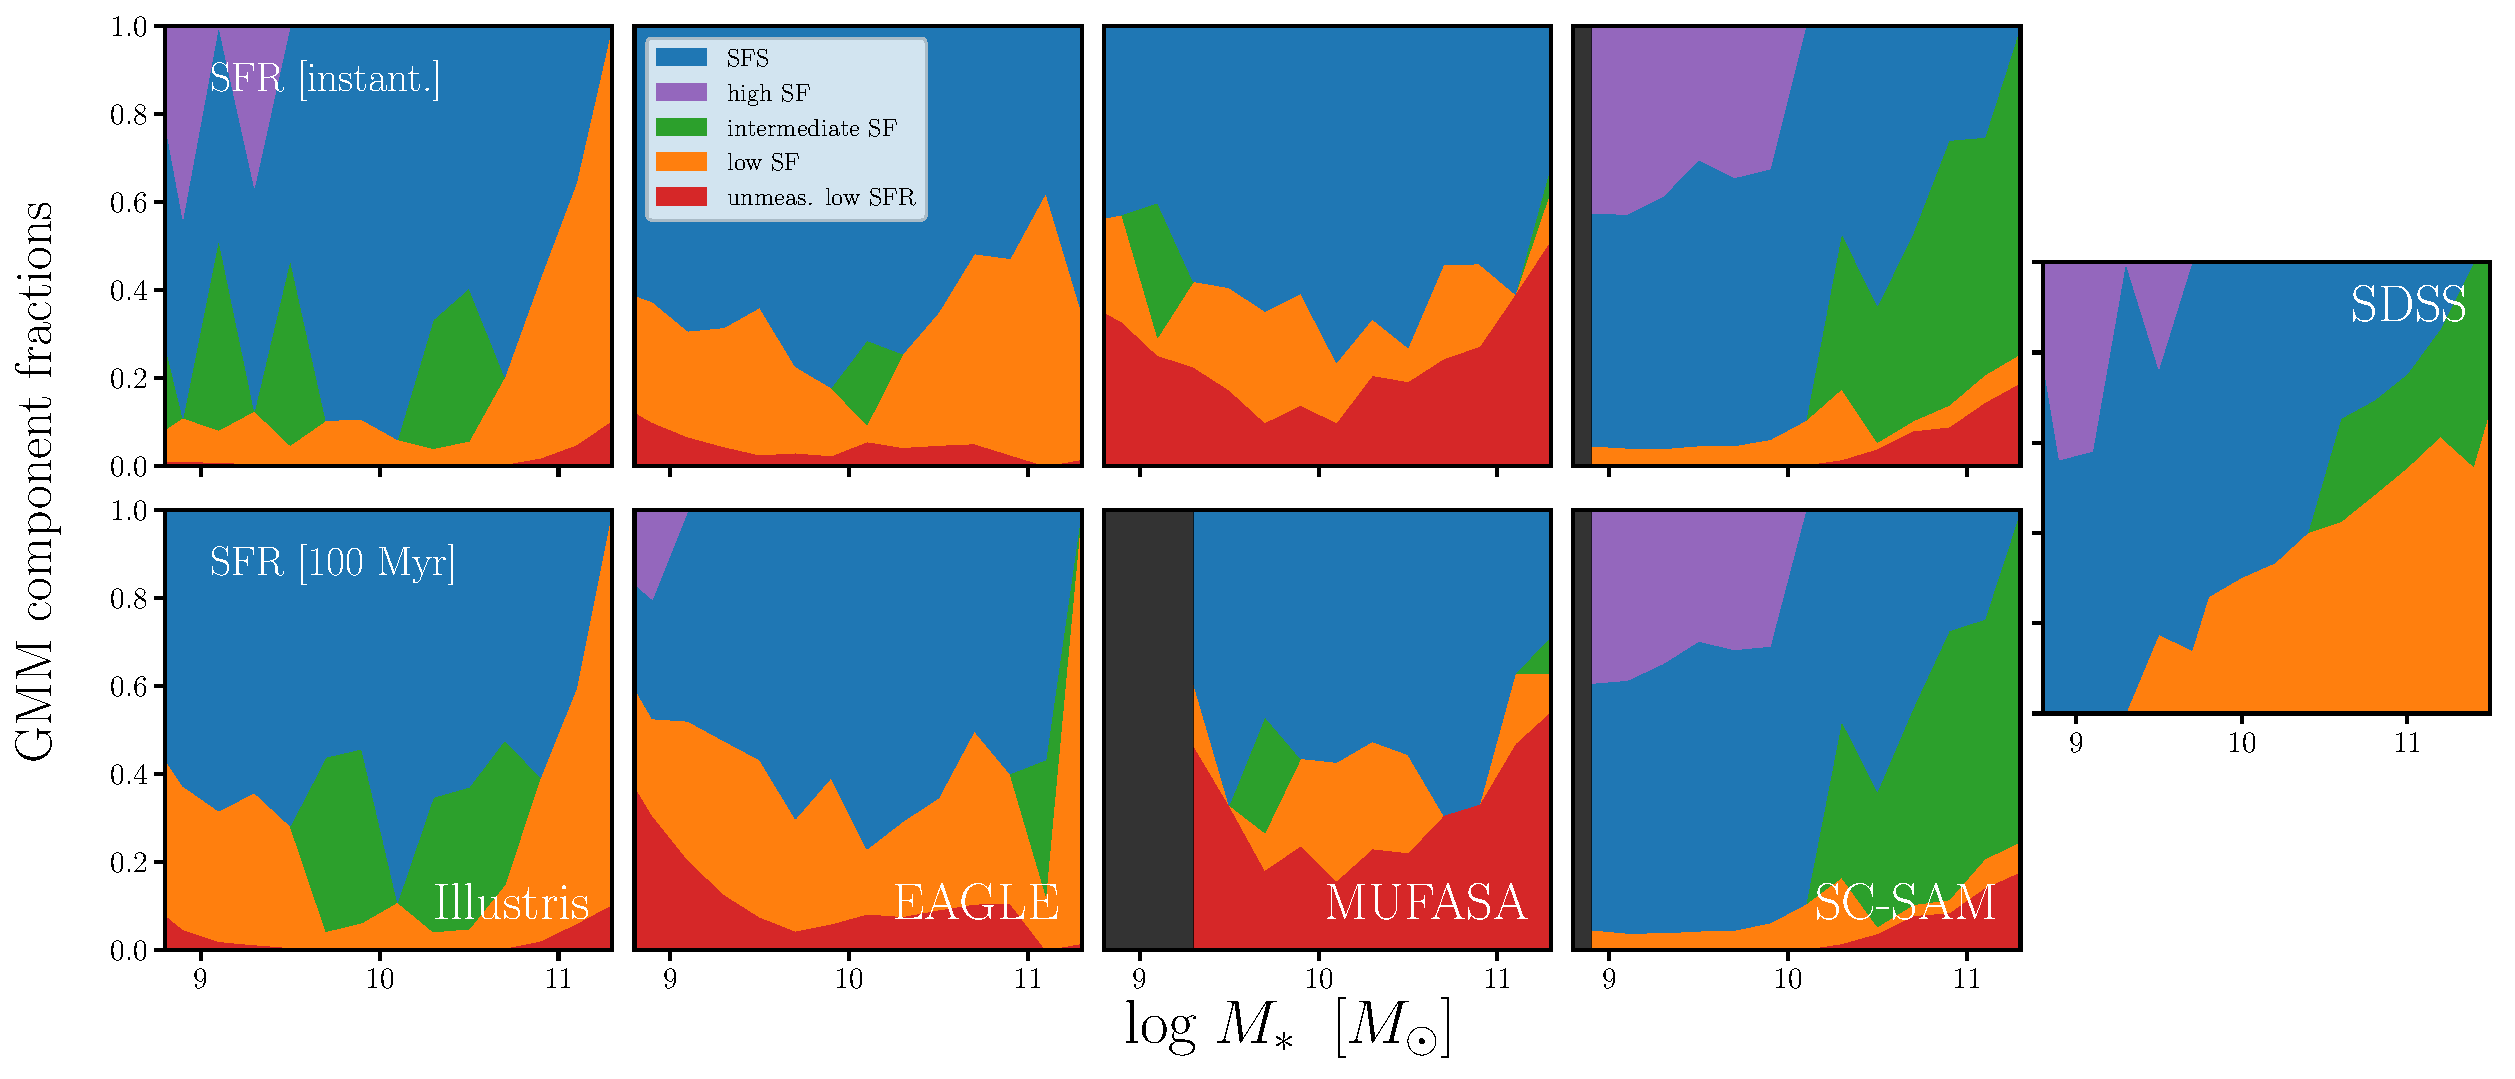
\includegraphics[width=\textwidth]{figs/GMMcomp_composition.pdf} 
\caption{Fractional contributions, $\pi_i$, of the best-fit GMM components from 
    our SFMS fitting of the central galaxies in the Illustris, EAGLE, MUFASA, 
    and Santa Cruz SAM simulations (left to right). We highlight the SFMS 
    component in blue, the quenched component in orange, galaxies with 
    SFR$=0$ in red, the transitioning components in green, and the star-burst
    components in purple. For reference, we include $\pi_i$ of the observed 
    centrals from SDSS and NSA in the rightmost panel. In all the simulations, 
    a significant fraction of central galaxies lie below the SFMS at 
    $M_* \lesssim 10^9 M_\odot$ in disagreement with observations. For the 
    hydrodynamic simulations, the SFMS fraction has little stellar mass dependence
    at $M_* < 10^{11}M_\odot$ unlike observations. Meanwhile, a number of similar 
    components are found between Santa Cruz SAM and observations: star-burst 
    components at low $M_*$ and transitioning components at high $M_*$. 
    } \label{fig:kandinsky}
\end{center}
\end{figure*}
%%%%%%%%%%%%%%%%%%%%%%%%%%%%%%%%%%%%%%%%%%

\subsection{Beyond the SFMS of simulated galaxies}
So far, we have focused solely on the SFMSs of our simulated 
galaxies---\emph{i.e.} $\bm{\theta}_\mathrm{SFMS} = \{\mu_\mathrm{SFMS}$ 
and $\sigma_\mathrm{SFMS} \}$. Our GMM fitting method, however, also determines 
$\bm{\theta}_i$ for components other than the SFMS. These GMM components 
provide extra features to compare our simulated galaxy samples and also offer 
interesting insights into the different populations in our simulated galaxy
samples. When we examine the mean and variance $\bm{\theta}_i$ of all the 
components from our fitting for our simulated galaxies we find correspondence 
between the components and the quiescent, transitioning, and star-burst galaxy 
populations (Figure~\ref{fig:sfmsfit_comps}). Similar to how we designated the 
SFMS component of the GMM, we designate the component with the lowest SFR as the quiescent 
component, the component with SFR in between the SFMS and the quiescent 
components as transitioning, and the component with SFR higher than the 
SFMS component as the star-burst component. In Figure~\ref{fig:sfmsfit_comps}, 
we mark the SFMS components in blue, quiescent components in orange, and 
the other components in green. 

All of the simulations have significant populations below the SFMS at all 
masses. The hydrodynamical simulations have relatively tight quiescent components 
${\sim}1\,\mathrm{dex}$ below the SFMS. The quiescent components of the 
Santa Cruz SAM, meanwhile, are much broader and extend below 
$\log\,\mathrm{SFR} = -4$. Regardless of their position and width, at low stellar
masses, the significant quiescent populations are in disagreement with 
observations~\citep{geha2012}, which find no isolated/central quenched 
galaxies below $M_*{\sim}10^9 M_\odot$. 
\begin{itemize}
    \item \todo{what's causing central galaxies to have low SFRs at $10^9M_\odot$?}
\end{itemize}
This discrepancy between simulations and observations, however, must be 
taken with a grain of salt. Both the environment and quenched classifications 
in \cite{geha2012} are defined differently than in the simulations. 
\cite{geha2012} classifies as a galaxy as quenched if it
does not have an $H\alpha$ emission and based on a $D_n 4000$ criteria. 
Furthermore, the isolation criteria of \cite{geha2012} is more 
stringent than the group finder at these mass scales.
%incept the idea for paper2. 

%Figure~\ref{fig:sfmsfit_comps} reveals components besides the SFMS and quiescent components. For instance, 
In Illustris and the Santa Cruz SAM, we find a number of components between 
the SFMS and quiescent components ---\emph{i.e.} transitioning galaxies. 
For Illustris, transitioning components 
are identified at $10^9 M_\odot < M_* < 10^{11}M_\odot$. For the Santa Cruz SAM, 
transitioning components are identified at $M_* > 10^{10} M_\odot$. We also 
identify components with SFRs above the SFMS. These \emph{star-burst} 
components are particularly evident in the Santa Cruz SAM, where a significant
star-burst population is observed at $10^9 M_\odot < M_* < 10^{10} M_\odot$. 
Besides the Santa Cruz SAM, we also find star-burst components at the lowest
stellar masses ($M_* < 10^9 M_\odot$) of the Illustris and EAGLE simulations 
for $100\,\mathrm{Myr}$ SFRs. 

The different components we identify using the GMM fitting allows us to make a 
number of interesting comparisons of the simulated galaxies. Overall
the galaxies from hydrodynamical simulations have similar components
and features in the SFR--$M_*$ data space. Besides the difference in the 
position and width of the SFMS, 
the only significant discrepancy is the transitioning components found in  
Illustris. 
%The transitioning components in the Illustris galaxies, however, help explain the tighter width of the SFMS compared to the other hydrodynamical simulations in Figure~\ref{fig:sfms_width}. 
Between the hydrodynamical simulations and the Santa Cruz SAM, however,
more significant differences are revealed by the non-SFMS components. 
\begin{itemize}
    \item \todo{Why is the SAM so different overall?}
    \item \todo{Why does Santa Cruz SAM have a broader SFR?} 
    \item \todo{Why does Santa Cruz SAM have star-bursts in "intermediate" stellar masses}
\end{itemize}

Another set of parameters we infer from our GMM fitting is the weight of the 
GMM components---$\pi_i$ in Eq.~\ref{eq:gmm}. Since we designated each component 
to a corresponding galaxy population, these weights correspond to the fractional
contribution of the different populations. For example, the weight of the 
quenched component is an estimate of the quiescent 
fraction~\citep[\emph{e.g.}][]{blanton2009, geha2012, hahn2015}. In 
Figure~\ref{fig:kandinsky} we present the fractional contribution, as a function 
of stellar mass, for all the components from our GMM fitting : SFMS (blue), 
quenched (orange), $\mathrm{SFR}=0$ galaxies (red), transitioning (green), 
and star-burst (purple). We present the uncertainties of $\pi_i$, estimated
through bootstrap resampling, in Figure~\ref{fig:fcomp_uncertainty} of 
Appendix~\ref{app:zerosfr}. 
For every simulation, a significant fraction of galaxies have SFR$=0$. 
In hydrodynamical simulations, a galaxy with $\mathrm{SFR}{=}0$ can have an 
SFR below the resolution limit, or have a \emph{true} $\mathrm{SFR}{=}0$ on 
the measured timescales (Appendix~\ref{app:zerosfr}). In the Santa 
Cruz SAM, all the $\mathrm{SFR}{=}0$ galaxies have truly no star formation 
on the timescales that we present here. Therefore, in both hydrodynamical 
and SAM simulations, the SFR$=0$ galaxies can be considered quiescent. 

The fractional contributions of the GMM components in Figure~\ref{fig:kandinsky}
reveal disagreements between our simulated galaxies and trends established
from observations---especially the hydrodynamical simulations. As we 
mentioned earlier, observations have established a stellar mass lower bound 
for isolated/central quenched galaxies~\citep{geha2012}. From Figure~\ref{fig:kandinsky}, 
we find significant quiescent populations at $M_* < 10^9 M_\odot$, confirming 
Figure~\ref{fig:sfmsfit_comps}. Treating SFR$=0$ galaxies as quiescent, the quiescent 
fraction for the EAGLE simulation is roughly $0.4$ at $10^9M_\odot$. 
Illustris with $100\,\mathrm{Myr}$ SFRs and MUFASA with instantaneous SFRs
have similarly high quiescent fractions. Even in the Santa Cruz SAM, we 
find a non-negligible ($\sim 10\%$) quiescent fraction at $10^9M_\odot$. 

Furthermore, at $M_* > 10^9M_\odot$, we find little stellar mass dependence in the 
fraction of high SFR components (SFMS and star-burst; blue and purple 
in Figure~\ref{fig:kandinsky}) in our hydrodynamical simulations at 
$M_* < 10^{11}M_\odot$. If we take the quiescent fraction to be 
$f_\mathrm{Q} = 1 - \sum_{\mathrm{high\,SFR}} \pi_i$, then the 
quiescent fraction of our central galaxies from hydrodynamical simulations 
have little stellar mass dependence over $10^9 < M_* < 10^{11} M_\odot$ ---
unlike $f_\mathrm{Q}$ measurements from~\cite{baldry2006,peng2010,hahn2015},
which all find significant stellar mass dependence in the quiescent/red fraction of 
isolated galaxies in SDSS. In this regards, the quiescent fraction of the 
Santa Cruz SAM is in good agreement with the isolated galaxy 
quiescent fraction from SDSS~\citep{baldry2006,peng2010,hahn2015}.

As we've discussed in this section, our SFMS fitting provides additional 
features, more than just the SFMSs, to compare different galaxy samples.
Moreover, the components identified by our fitting method offers insight
into the distinct galaxy populations of our simulations. Based on the 
non-SFMS components/populations, we find consistency among the hydrodynamical
simulations in SFR--$M_*$ space, but not with the Santa Cruz SAM. When we
compare to trends in the literature, we find that all of the simulations 
have a significant fraction of low SFR (quenched) central galaxies at 
$M_* \lesssim 10^9M_\odot$---in disagreement with observations. In particular, 
the hydrodynamical simulations, at intermediate stellar masses 
$M_* \lesssim 10^{11}M_\odot$, do not reproduce the quiescent fractions from 
observations. 

\subsection{Comparing to Observations}
Our data-driven GMM SFMS fitting provides a principled way to compare 
galaxy populations through the major features in the data-space. These 
comparisons have so far revealed a number of agreements and discrepancies
among the central galaxies in our simulations. The ultimate goal of 
these simulations, however, is to reproduce the observations, which means
we ultimately want to compare them to observations. In this section, we 
extend our GMM SFMS fitting to the observed galaxy sample from SDSS and NSA
and compare our simulated galaxies to observation.

We first focus on the best-fit SFMS of our SDSS and NSA central galaxies
in the top right panels of Figure~\ref{fig:sfmsfit_inst} and~\ref{fig:sfmsfit_100myr}. 
Similar to the Illustris, EAGLE, and Santa Cruz SAM simulations, the SFR of 
the SFMS monotonically increases with $M_*$. The SFMS has no turnover like
MUFASA's. Overall, the SDSS and NSA SFMS is shallower and has a lower amplitude 
than the SFMSs of our simulations. \todo{chang: any reasons why we see this 
discrepancy from the simulation side?}

Looking beyond the SFMS, the other components of the SDSS and NSA central 
galaxy population further highlight the disagreements between the 
simulations and observation from the previous section (Figure~\ref{fig:kandinsky}). 
At $M_* \lesssim 10^9M_\odot$, we find no quenched population, in agreement 
with~\cite{geha2012} and in disagreement with the simulations. Furthermore, 
in agreement with measurements in the literature, we find significant $M_*$
dependence in the quiescent fraction, which the hydrodynamic simulations do 
not find. Aside from the low stellar mass quenched population, the components 
of the Santa Cruz SAM simulation are in good agreement with the SDSS and NSA 
components. They both identify star-burst populations at low masses and 
significant transitioning populations from $M_* > 10^{10}M_\odot$.  

%The SDSS samples show a SFR-$M_*$ relation that is best fitted by \emph{one} Gaussian at lower masses, unlike any of the simulations. This is noteworthy even though the low-mass sample is far from volume-complete and especially many low-SFR galaxies may be missed at lower masses.
%\item[-] The observations show a very well defined, and for higher mass bins quite narrow, low-SFR population, with a small intermediate third population for only three mass bins. The low-SFR population is more narrow and generally with the mean at slightly lower SFR than for all three hydro simulations. It is located in between the intermediate and low-SFR populations of the SAM.

The comparison we make between our simulations and observations so far in 
this section only scratches the surface. However, we deliberately refrain 
from a more detailed comparison due to the limitations of such a comparison. 
The main bottleneck stems from the fact that the SFRs and $M_*$, the main
galaxy properties considered in this paper, are defined and measured 
differently in simulations versus observations. SFRs from the SDSS and 
NSA catalogs are measured using a combination of $H\alpha$ and $D_n 4000$. 
Although we choose the SFR timescales to best reflect this observed SFR, 
as \cite{speagle2014} find even for the same SDSS galaxies, different SFR 
indicators can produce large discrepancies in the slope and amplitude of 
the SFMS. Therefore, for further scrutiny we require a more apples to apples 
comparison. In the next paper we will bring this comparison on a more equal 
footing by deriving star formation rates from mock observations of the 
simulated galaxies (Starkenburg et al. in prep.).

%\todo{TKS: Compare to Speagle2014 combined dataset fits and discuss with respect to the large discrepancy they note in MS-slopes for the SDSS sample of $~0.4$ dex. This is partly due to using different SFR indicators (nice segue to the 2nd and 3rd papers), but not completely}
%comparison to observations are complicated by a number of factors.  First the SFRs and stellar masses of observations are defined by kcorrect  and emission lines and dn4000. While our SFR timescales were chosen to best  reflect the observed SFR, it's still not an apples to apples comparison.  Second, the stellar mass and SFRs of observed galaxies have uncertainties  associated to them. If unaccounted for, these uncertainties will impact the  components recovered from the GMM fitting and ultimately the SFMS fits. 
%All of the points in this subsection are severely affected by the different ways that SFR (and $M_*$) are measured in the observations and the simulations. 

\section{Summary and Conclusions} \label{sec:summary}
conclusion!

\section*{Acknowledgements}
It's a pleasure to thank
	Shirley~Ho, 
	Emannuel~Schaan, 
    \todo{insert others} 
for valuable discussions. 
This material is based upon work supported by the U.S. Department
of Energy, Office of Science, Office of High Energy Physics, under
contract No. DE-AC02-05CH11231.
\appendix
%%%%%%%%%%%%%%%%%%%%%%%%%%%%%%%%%%%%%%%%%%
% Figure j 
%%%%%%%%%%%%%%%%%%%%%%%%%%%%%%%%%%%%%%%%%%
\begin{figure}
\begin{center}
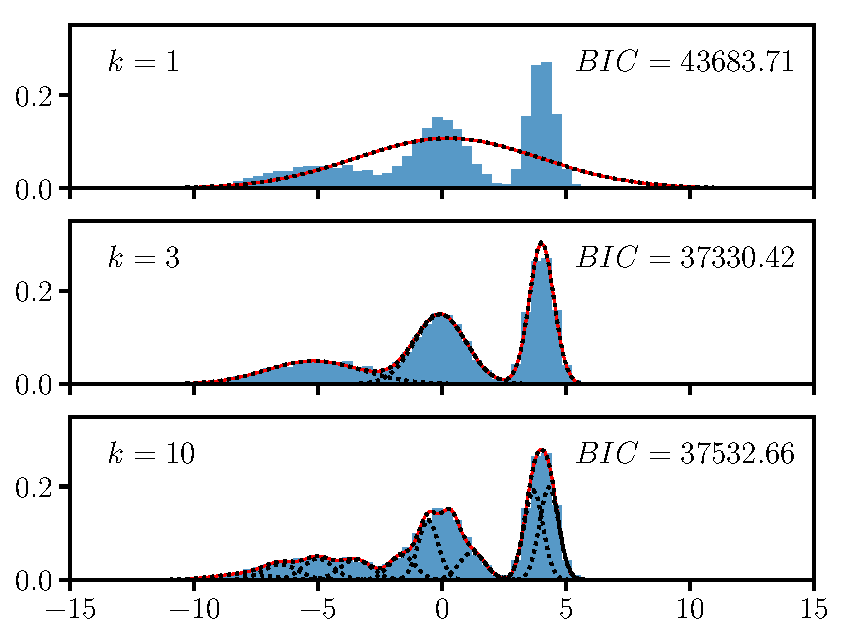
\includegraphics[width = 0.475\textwidth]{figs/GMM_pedagog.pdf} 
\caption{A pedagogical illustration of Gaussian mixture density estimation. 
We use GMMs with $k = 1$ (top), $3$ (middle), $10$ (bottom) components to estimate 
the distribution of data (blue) drawn from three Gaussian distributions. The GMM 
outputs of the EM algorithm are plotted in red with dotted lines representing each 
of their components. We also include the BIC of the GMMs, which we use to select 
the number of components $k$. Of the three panels, $k=3$ has the lowest BIC and 
therefore best represents the data according to our selection 
scheme. \todo{move to appendix}} \label{fig:gmm_pedagog}
\end{center}
\end{figure}
%%%%%%%%%%%%%%%%%%%%%%%%%%%%%%%%%%%%%%%%%%

%%%%%%%%%%%%%%%%%%%%%%%%%%%%%%%%%%%%%%%%%%
% Figure  
%%%%%%%%%%%%%%%%%%%%%%%%%%%%%%%%%%%%%%%%%%
\begin{figure*}
\begin{center}
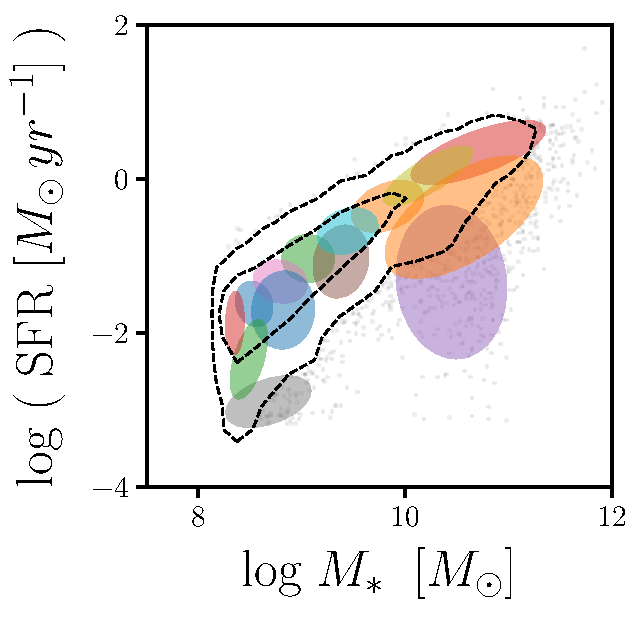
\includegraphics[width = 0.45\textwidth]{figs/SFRMstar_2Dgmm.pdf} 
\caption{Two-dimensional GMM fit to the SFR-$M_*$ relation of central galaxies
of the EAGLE simulation. The two-dimensional GMM fitting is an extension of the 
SFMS fitting method we describe in Section~\ref{sec:sfmsfit}. The colorful shaded
ellipses over-plotted on the SFR-$M_*$ relation (black) are the Gaussian components 
of the best-fit GMM. Although, identifying the SFMS from these Gaussian components
is difficult, the 2D GMM is effective in capturing the features of the SFR-$M_*$ 
relation and provides a good way comparing SFR-$M_*$ relations from different data.
} \label{fig:2dgmm}
\end{center}
\end{figure*}
%%%%%%%%%%%%%%%%%%%%%%%%%%%%%%%%%%%%%%%%%%

\section{Gaussian Mixture Models: 1D and Beyond} \label{app:gmm}
So far we have assumed that one, two, or three populations would describe galaxies in the SFR--$M_*$ plane well. We have checked whether the possibility of adding more than three Gaussians in the GMM shows that more populations are present. This is the case only for the Santa Cruz semi-analytic model, where in a number of bins the presence of 4, 5, or (in one case) 6 Gaussians is preferred. In almost all cases the added Gaussians have low weight and form effectively additional intermediate populations. For both Illustris and EAGLE there is only one mass bin where a fourth population would be preferred. For all other mass bins in all the hydrodynamical simulations, and all mass bins in the SDSS 3 or less Gaussians are preferred.


In addition to identifying the SFMS, the GMM fitting method described above can 
be extended to describe the entire SFR-$M_*$ relation using a two-dimensional 
GMM. In Figure~\ref{fig:2dgmm}, we compare the instantaneous SFR to $M_*$ relation 
of central galaxies in the EAGLE simulation with the best-fit two-dimensional GMM. 
The over-plotted shaded ellipses represent the two-dimensional Gaussian components
of the best-fit GMM. Overall the best-fit 2D GMM captures the features in the 
EAGLE SFR-$M_*$ relation. It also provides a straightforward way of comparing 
different SFR-$M_*$ relations. However, as Figure~\ref{fig:2dgmm} illustrates, 
specifically identifying the SFMS using the two-dimensional model is more 
challenging. Therefore in this paper, we do not discuss the 2D GMM further. 

\section{SFR Resolution Effects} \label{app:zerosfr}
In our analysis, we consistently derive SFRs for all of our simulated
galaxies on two timescales: instantaneous and averaged over 
$100\,\mathrm{Myr}$ (Section~\ref{sec:galsims}). For our hydrodynamic 
simulations, SFR averaged over $100\,\mathrm{Myr}$ is derived using 
the formation times of the star particles in the simulation. This means 
that both the \todo{spatial(?)} and temporal resolutions of the 
simulations cause resolution effects in the $100\,\mathrm{Myr}$ SFR. 
More specifically, in Illustris, EAGLE, and MUFASA $100\,\mathrm{Myr}$ 
SFR has a resolution of $\Delta_\mathrm{SFR} = 0.016$, $0.018$, and 
$0.182\,M_*/\mathrm{yr}$, respectively. 
\todo{a sentence about why MUFASA's resolution is an order of magnitude higher}.

% describe the impact of resolution effect more concretely 
Although for galaxies with high $100\,\mathrm{Myr}$ SFR, the resolution 
of $\Delta_\mathrm{SFR}$ does not have a significant impact, for low SFR
galaxies, the fact that their SFR is actually within the range 
$[\mathrm{SFR}, \mathrm{SFR}+\Delta_\mathrm{SFR}]$ has a significant 
impact. For example, at the most low SFR end, galaxies, which would 
have SFR < $\Delta_\mathrm{SFR}$, are derived to have SFR$=0$. These 
galaxies, consequently, cannot be included in the
$\log\,\mathrm{SFR}$--$\log\,M_*$ plane or the SFMS fitting. In
Figure~\ref{fig:zerosfr_res}, we present the impact of this resolution 
effect on the $P(\log\,\mathrm{SSFR})$ distributions of our 
hydrodynamical simulations in two stellar mass bins. In black, we 
plot the $P(\log\,\mathrm{SSFR})$ distributions using the 
$100\,\mathrm{Myr}$ SFRs \emph{with} resolution effects --- galaxies 
with SFR$=0$ are not included in this distribution. In blue, we 
plot the $P(\log\,\mathrm{SSFR})$ distributions of the same galaxies, 
but with SFR sampled uniformly within the range 
$[\mathrm{SFR}, \mathrm{SFR}+\Delta_\mathrm{SFR}]$. Uncertainties 
for the blue $P(\log\,\mathrm{SSFR})$ is derived from repeating process of
sampling the SFR $100$ times. 

%%%%%%%%%%%%%%%%%%%%%%%%%%%%%%%%%%%%%%%%%%
% Figure 
%%%%%%%%%%%%%%%%%%%%%%%%%%%%%%%%%%%%%%%%%%
\begin{figure*}
\begin{center}
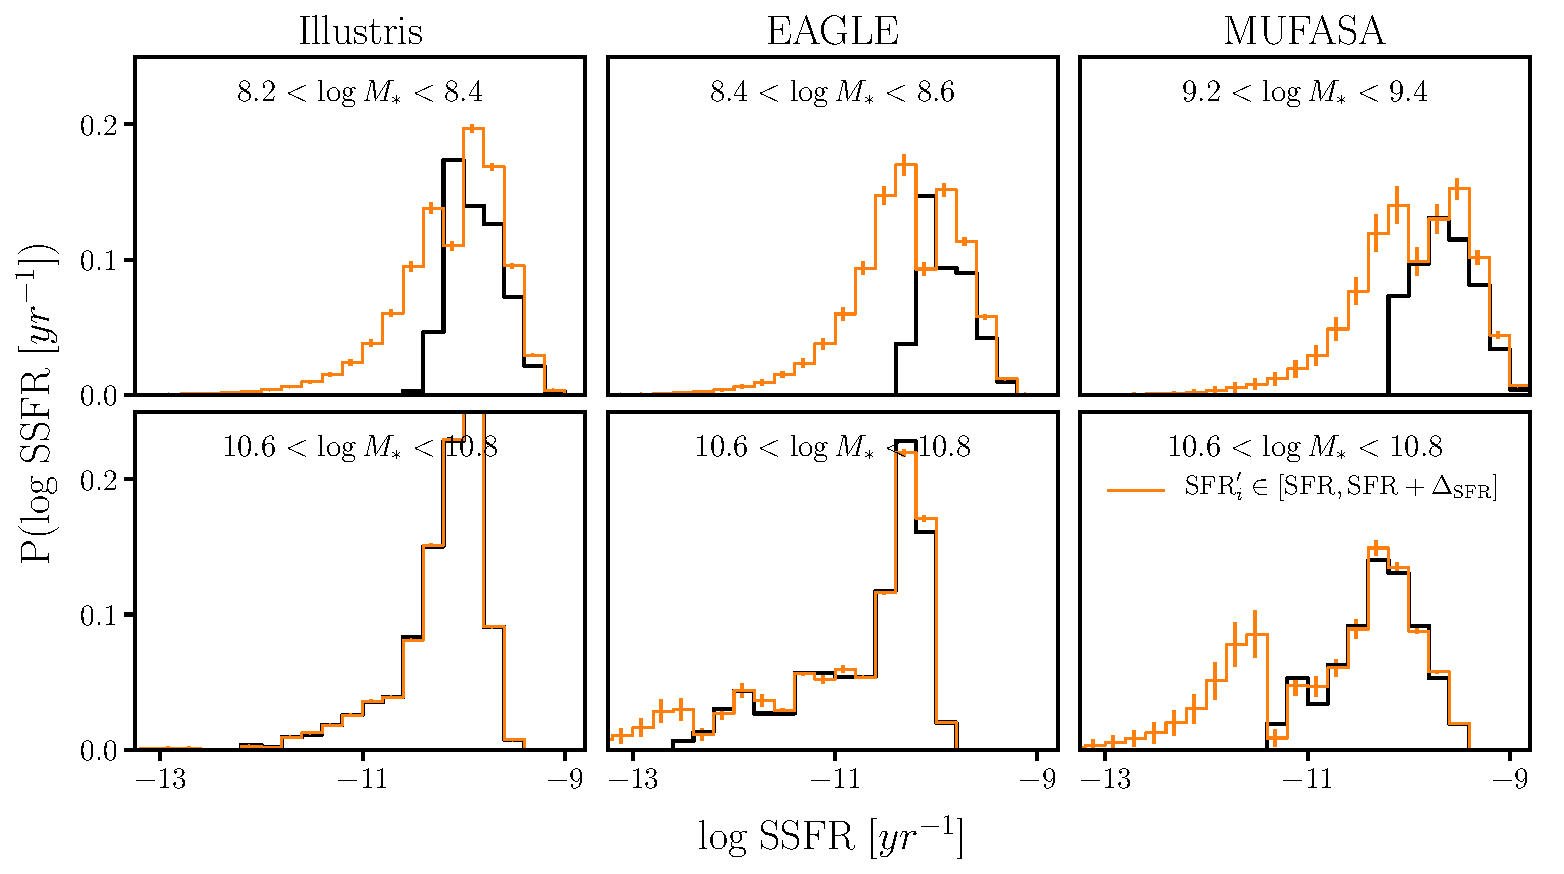
\includegraphics[width=0.9\textwidth]{figs/Pssfr_res_impact.pdf} 
\caption{The impact of SFR resolution and galaxies with SFR$=0$, on 
the SSFR distribution, $P(\mathrm{SSFR})$, of Illustris, EAGLE, and 
MUFSAS simulations. We plot $P(\mathrm{SSFR})$ with $\mathrm{SFR} = 0$
galaxies in blue and $P(\mathrm{SSFR})$ without $\mathrm{SFR} = 0$ 
galaxies in black. The uncertainties of $P(\mathrm{SSFR})$ is obtained 
from re-sampling the SFR of each galaxy based on the SFR resolution, 
as described in  Appendix~\ref{app:zerosfr}. For each simulation, we 
present two distinct stellar mass bins to illustrate the impact at low 
and high $M_*$.
} 
\label{fig:zerosfr_res}
\end{center}
\end{figure*}
%%%%%%%%%%%%%%%%%%%%%%%%%%%%%%%%%%%%%%%%%%

%%%%%%%%%%%%%%%%%%%%%%%%%%%%%%%%%%%%%%%%%%
% Figure 
%%%%%%%%%%%%%%%%%%%%%%%%%%%%%%%%%%%%%%%%%%
\begin{figure*}
\begin{center}
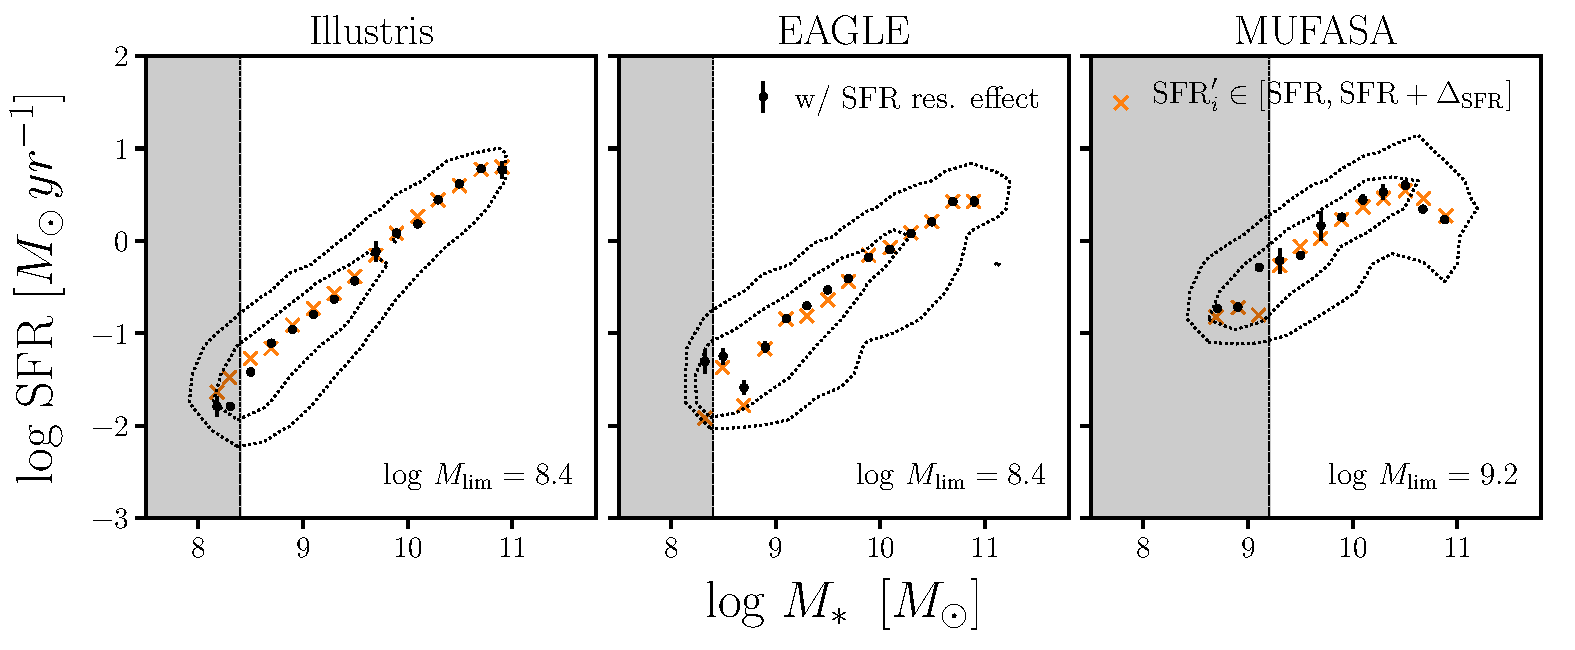
\includegraphics[width=0.8\textwidth]{figs/Mlim_res_impact.pdf} 
\caption{Resolution effects of hydrodynamical simulations (Illustris, 
EAGLE, and MUFASA) impact our SFMS fitting for SFR averaged over 
$100\,\mathrm{Myr}$ at low stellar mass. We therefore determine stellar
mass limits based on the discrepancy between the SFMS fits neglecting 
the resolution limit (black) and fits trying to include the resolution 
limit by re-sampling the SFRs (orange; Appendix~\ref{app:zerosfr}). For
Illustris, EAGLE, and MUFASA we set $\log M_\mathrm{lim} = 8.4, 8.6$, and 
$9.4$, respectively.} 
\label{fig:mlim_res}
\end{center}
\end{figure*}
%%%%%%%%%%%%%%%%%%%%%%%%%%%%%%%%%%%%%%%%%%

%%%%%%%%%%%%%%%%%%%%%%%%%%%%%%%%%%%%%%%%%%
% Figure 
%%%%%%%%%%%%%%%%%%%%%%%%%%%%%%%%%%%%%%%%%%
\begin{figure*}
\begin{center}
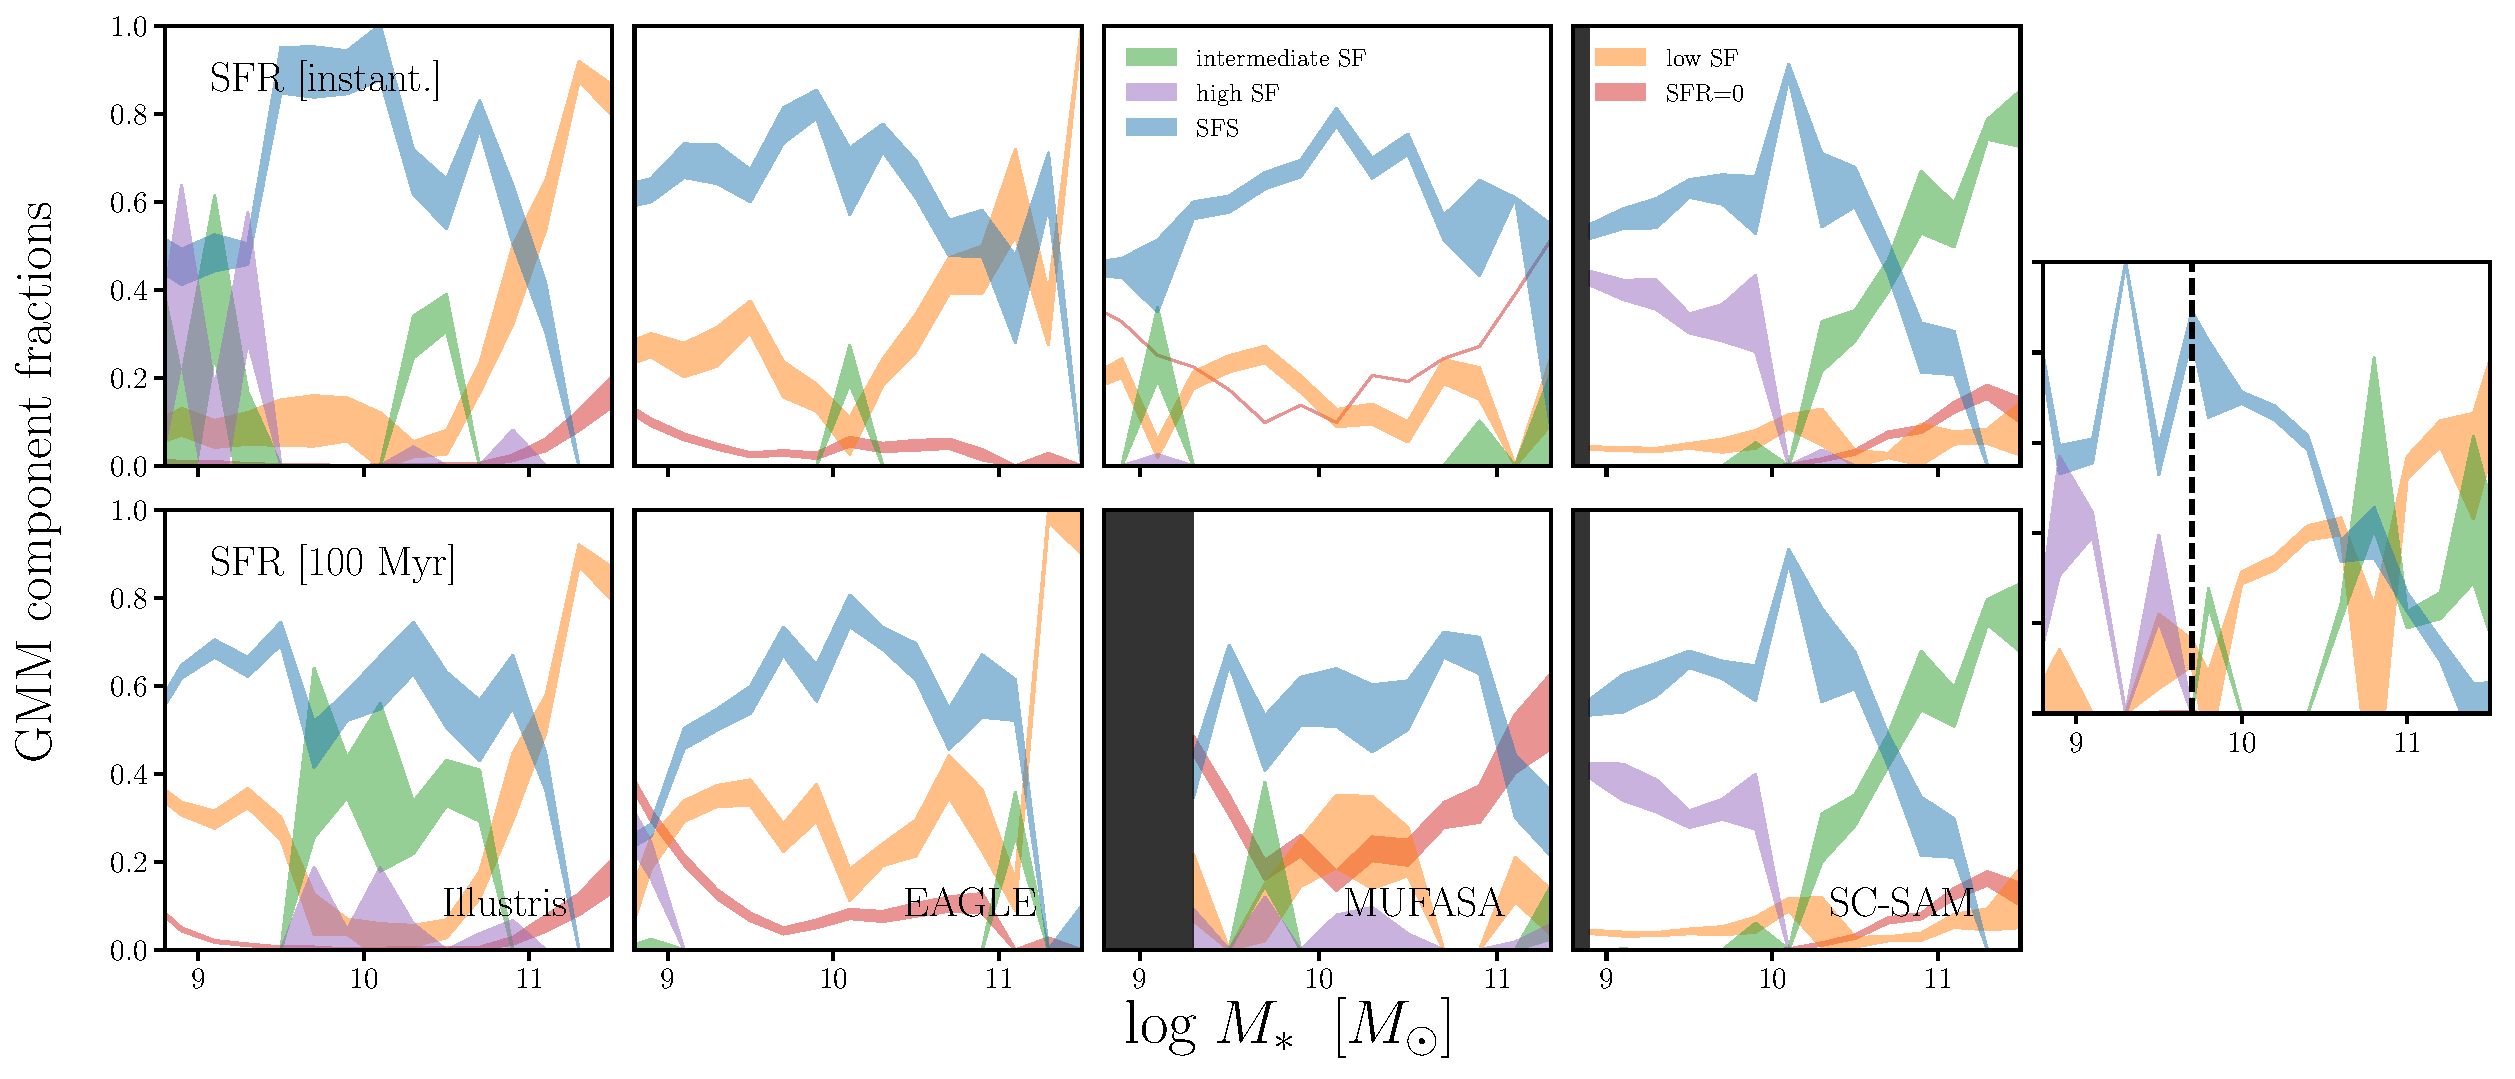
\includegraphics[width=0.9\textwidth]{figs/GMMcomp_comp_uncertainty.pdf} 
\caption{
} \label{fig:fcomp_uncertainty}
\end{center}
\end{figure*}
%%%%%%%%%%%%%%%%%%%%%%%%%%%%%%%%%%%%%%%%%%
\bibliographystyle{aasjournal}
\bibliography{paper1}
\end{document}